\documentclass[submit]{ipsj}
%\documentclass{ipsj}

%\usepackage{graphicx}
%\usepackage[dvipdfmx]{graphicx,color}
%\usepackage[dvips]{graphicx}
\usepackage[dvipdfmx]{graphicx}
\usepackage{latexsym}
\usepackage{url}
\usepackage{listings}
\usepackage{multirow}
\usepackage{xcolor}
\usepackage{colortbl}


\newcommand{\todo}[1]{\colorbox{yellow}{{\bf TODO}:}{\color{red} {\textbf{[#1]}}}}

%ここからソースコードの表示に関する設定
\definecolor{darkgray}{rgb}{.4,.4,.4}
\definecolor{purple}{rgb}{0.65, 0.12, 0.82}

\lstdefinelanguage{JavaScript}{
  keywords={typeof, new, true, false, catch, function, return, null, catch, switch, var, if, in, while, do, else, case, break},
  keywordstyle=\color{blue}\bfseries,
  ndkeywords={class, export, boolean, throw, implements, import, this},
  ndkeywordstyle=\color{darkgray}\bfseries,
  identifierstyle=\color{black},
  sensitive=false,
  comment=[l]{//},
  morecomment=[s]{/*}{*/},
  commentstyle=\color{purple}\ttfamily,
  stringstyle={\small\ttfamily},
  morestring=[b]',
  morestring=[b]"
}

\lstset{
  basicstyle={\ttfamily},
  identifierstyle={\small},
  commentstyle={\smallitshape},
  keywordstyle={\small\bfseries},
  ndkeywordstyle={\small},
  stringstyle={\small\ttfamily},
  frame={tb},
  breaklines=true,
  columns=[l]{fullflexible},
  numbers=left,
  xrightmargin=0zw,
  xleftmargin=3zw,
  numberstyle={\scriptsize},
  stepnumber=1,
  numbersep=1zw,
  lineskip=-0.5ex
}
%ここまでソースコードの表示に関する設定

\def\Underline{\setbox0\hbox\bgroup\let\\\endUnderline}
\def\endUnderline{\vphantom{y}\egroup\smash{\underline{\box0}}\\}
\def\|{\verb|}

\setcounter{巻数}{59}
\setcounter{号数}{1}
\setcounter{page}{1}


\受付{2016}{3}{4}
\再受付{2015}{7}{16}   %省略可能
\再再受付{2015}{7}{20} %省略可能
\再再受付{2015}{11}{20} %省略可能
\採録{2016}{8}{1}




\begin{document}


\title{JavaScriptライブラリのテストコード変更に基づく\\後方互換性を損失するバージョン検出}

\etitle{Detecting Software Library Version\\with Backward Compatibility Loss based on Test Code Changes}

\affiliate{WA}{和歌山大学システム工学部\\
Wakayama University, Faculty of Systems Engineering, Sakaedani 930, Wakayama-city 640-8510, Japan}


 \paffiliate{YAHOO}{LINEヤフー株式会社\\LY Corporation}

\author{伊原 彰紀}{Akinori Ihara}{WA}[ihara@wakayama-u.ac.jp]
\author{前川 大樹}{Daiki Maekawa}{WA}[maekawa.daiki@g.wakayama-u.jp]
\author{松田 和輝}{kazuki Matsuda}{WA,YAHOO}[matsuda.kazuki@g.wakayama-u.jp]

\begin{abstract}
%ソフトウェア開発では,ライブラリと呼ばれる再利用可能なソースコードを利用することで,開発者が一部の機能を実装する必要がなくなり,開発効率が向上する.多くのソフトウェアで利用されるライブラリの開発者は,ライブラリのバージョンを更新時にクライアントソフトウェアに影響を与えないように,ライブラリ更新後に後方互換性を意図せず損失しないことが求められる.しかし,軽微なバグ修正などにより,ライブラリ開発者が意図しない部分でソースコードの動作が変わり,ライブラリの後方互換性が損失することがある.
本研究では,「ライブラリの変更に伴いテストコードを変更したバージョンでは後方互換性を損失している」と仮説を立て,ライブラリのテスト変更有無に基づいて後方互換性の有無を判断する実証的分析を行った.さらにテストコードの変更内容に基づき,後方互換性を損失するバージョンの検出ツールを開発した.その結果,本手法は分析対象とするライブラリバージョン更新で後方互換性を損失している割合よりも高い精度で検出することができた.

%その結果,テストの変更内容に基づき後方互換性を損失する51\%のライブラリバージョンの特定に成功した.
\end{abstract}


\begin{jkeyword}
ソフトウェアライブラリ,後方互換性,ソースコード静的解析
\end{jkeyword}

\begin{eabstract}
% In software development, developers do not implement some functions by using software libralies, then improves development efficiency. Library developers should avoid unintentional loss of backward compatibility after library updates because client software is affected when library versions are updated.
% However,  backward compatibility of the library might be loss when library developers change the source code by minor bug fixes. 
This study hypothesized ``When library developers change test codes in new library version, the library version contains the loss of backward compatibility'' and conducted an empirical analysis to predict whether or not the new library version with test code changes contains the loss of backward compatibility. Furthermore, this study developed an automatic detection tool for loss of backward compatibility based on the context of code changes. As a result, our approach successfully detected backward compatibility loss with higher accuracy than its rate in our target library version updates.
%we successfully identify 51\% library versions with backward compatibility loss based on the context of code changes.
\end{eabstract}

\begin{ekeyword}
Software library, Backward compatibility, Statistic code analysis
\end{ekeyword}

\maketitle

%%%%%%%%%%%%%%%%%%%%%%%%%%%%%%%
\section{はじめに}
%%%%%%%%%%%%%%%%%%%%%%%%%%%%%%%

ソフトウェア開発では,自身が実装するソースコードの機能の一部として,自身や他の開発者が作成したライブラリを再利用することがある.
%ライブラリは,汎用性の高いプログラムを再利用可能な形式でまとめたものであり,定型的な処理の実装を実現するためソフトウェア開発を効率化することができる.
ライブラリは,ライブラリを使用するクライアントソフトウェア(以降,クライアント)とそれぞれ独立して開発される.開発によってライブラリに変更が加えられた場合,クライアント開発者は必要に応じて,クライアントの開発に用いているライブラリのバージョンを更新する.
%これらの関係を図\ref{fig:clientLibrary}に示す.

%\begin{figure}[h]
%  \vspace{1zh}
%  \centering
%  \includegraphics[width=0.95\linewidth]{fig/client-library.pdf}
%  \caption{クライアントとライブラリの関係}
%  \label{fig:clientLibrary}
%\end{figure}

%クライアント開発者が依存ライブラリを更新する際,新しいバージョンに含まれる変更が脆弱性の修正などクライアントにとって重要な変更である場合,クライアント開発者は依存ライブラリのバージョン更新を余儀なくされることも多い.
%一方で
ライブラリの更新には,これまでの使用方法が変わるような既存機能の仕様変更を含むことがある.このような変更を含むバージョンに更新すると,クライアントの動作の変化やエラーの原因になることがある.
このようにクライアントの既存機能に影響を与えるライブラリの変更は破壊的であると表現され,その変更は破壊的変更 (Breaking Change) と呼ばれる.特に,ライブラリの更新後のバージョンが,更新前のバージョンとの互換性を失うことを後方互換性の損失と呼ぶ.
ライブラリ開発者は,ライブラリのバージョンが後方互換性を損失しているか否か,つまり新しいバージョンの適用によってクライアントが影響を受ける可能性の有無を,バージョン名によってクライアント開発者に伝達する.
%クライアント開発者は依存ライブラリを更新する際に,クライアントがライブラリの変更による影響を受けるか否かをあらかじめ把握しておくために,バージョン更新後の依存ライブラリに破壊的変更が含まれているか否かを確認する必要がある.
%このような問題に対してライブラリ開発者は,ライブラリのバージョン更新の際に変更内容を確認し,バージョン名などによってクライアント開発者に破壊的変更の有無を伝達することがある.
しかし,ライブラリ開発者による後方互換性の損失を含むか否かは目視によって判断されるため,後方互換性の損失がないと誤って判断されたバージョン更新でクライアントの既存機能に影響を与えることがある.
%ライブラリを利用した開発において,ライブラリの後方互換性の判断が困難なために,脆弱性の修正などといった重要な変更がクライアントに適用されないことがある.
%このような課題の解決に向けて,ライブラリの後方互換性を判断する研究が進められている.
%既存研究は,ライブラリの変更内容の分析\cite{Efficient_Static_Checking}や,クライアントの動作を検証するテストに破壊的変更の影響が表れることを利用した手法\cite{Using_Others_Tests}による,後方互換性の判断方法を提案している.
特に,動的型付け言語であるJavaScript言語では,静的解析によって後方互換性の判断ができない場合があり,さらに数多くのクライアントテストを用いても後方互換性の損失による影響が表れない場合があるため,後方互換性の正確な判断は困難である\cite{type-regression-testing}\cite{model-based-testing}.

本研究では,ライブラリのテストコードの変更に基づき後方互換性の損失の有無を予測する実証的分析を行う.
%後方互換性の判断を困難にする要因の一つであるプログラムの動的な処理は,ライブラリに付属するテストに記述されている.
テストコードはライブラリの動作検証を目的に実装されるため,ライブラリの機能変更で期待する振る舞いが変われば,それに合わせてテストコードにおける検証内容も変更する.このようなテストコードに影響を与えるライブラリの変更は,クライアントにも影響を与える破壊的な変更であると考える.
本研究では,「ライブラリの変更に伴いテストコードを変更したバージョンでは後方互換性を損失している」と仮説を立て,2つの分析に取り組む.

\begin{itemize}
\item[分析1:] ライブラリのバージョン更新でテストコードも変更しているとき,当該バージョンには後方互換性の損失も含むか否か明らかにする(\ref{sec:prepare}章).
\item[分析2:] 後方互換性の損失に伴い変更されたテストコードの内容を明らかにし,変更内容に基づき後方互換性の損失を含むか否かを明らかにする(\ref{sec:contentAnalysis}章,\ref{chap:rq2}章).
\end{itemize}

各分析では人気の高い1,955件のJavaScriptライブラリを対象に行い,各ライブラリを使用するクライアントのテストコードが失敗するか否かによって後方互換性の有無を検証する.

以降,本論文では\ref{sec:backward-compatibility}章でライブラリ開発における後方互換性の損失によるクライアントへの影響,および関連研究について述べ,本研究の立ち位置を説明する.\ref{sec:hypothesis}章で本研究の仮説を述べ,\ref{sec:analyticalMethod}章で仮説をもとにした分析手法を述べる.\ref{sec:prepare}章では,分析1の方法およびその結果について述べる.\ref{sec:contentAnalysis}章では,後方互換性の損失にともなうテスト変更の内容の調査を述べ,\ref{chap:rq2}章では,テスト変更の内容に基づく後方互換性の損失の検出方法およびその結果について述べる.\ref{sec:validity}章では本研究の妥当性を述べ,\ref{sec:conclusion}章で本研究をまとめる.

%%%%%%%%%%%%%%%%%%%%%%%%%%%%%%%
\section{後方互換性の損失}\label{sec:backward-compatibility}
%%%%%%%%%%%%%%%%%%%%%%%%%%%%%%%

\subsection{後方互換性の損失の原因}
ライブラリが後方互換性を損失する原因の一つに,ライブラリが提供するAPIの振る舞いの変更がある.メソッド,シグネチャ,例外,入出力データ形式など,APIの振る舞いの変更はクライアントに影響を与える可能性が高い.APIの機能拡張やバグ修正であっても,拡張された機能が存在しないことや,壊れている動作に依存していた場合,クライアントがエラーを引き起こす原因になる.一方,提供するAPIの追加や,ライブラリの内部で使用されるモジュールの変更では一般的にクライアントが影響を受けることは少ない.Java言語では,privateアクセス修飾子等を利用することで,クライアントに影響を与えることなく,ライブラリの内部で利用するモジュールを変更することができる.しかし,JavaScript言語ではAPIとしてクライアントに提供するモジュール,または内部で使用するモジュールかを明確に定義することが少ない.その結果,ライブラリ開発者が内部で使用するモジュールと考え,変更していたとしても,当該モジュールを使用する多数のクライアントが変更の影響を受けることもある.ユーザインターフェースを構築するライブラリReactの15.3.2から15.4.0へのマイナーアップデート\footnote{\url{https://github.com/facebook/react/compare/v15.3.2...v15.4.0}}では,react/lib/ReactMountモジュールを刷新する変更が行われた.ライブラリ開発者は,内部使用のみを意図していたが,当該モジュールを使用する多数のクライアントが変更の影響を受けた事例である\footnote{\url{https://github.com/rekit/rekit/issues/16}}.

\subsection{クライアントに与える影響}
JavaScriptライブラリの後方互換性の損失がクライアントに与える影響を調査した研究\cite{impact-analysis-for-clients}では,npm\footnote{\url{https://www.npmjs.com/}}から384件のクライアントを調査し,約12\%が後方互換性の損失による影響を受けたことを示している.また,後方互換性を損失した全64件のリリースのうち,約44\%がマイナーリリースとパッチリリースであり,ライブラリ開発者がバージョン名のみで後方互換性の有無を判断できていなかった.ライブラリのバージョン名に誤った値が付与されている場合,クライアント開発者が後方互換性を維持することを期待してライブラリバージョンを適用し,エラーを引き起こしてしまうことになる.2016年12月,デバッグ用のAPIを提供するライブラリdebugの2.3.3から2.4.0へのマイナーアップデート\footnote{\url{https://github.com/debug-js/debug/compare/2.3.3...2.4.0}}では,ソースコード中に単純なスペルミスによるバグが混入し\footnote{\url{https://github.com/debug-js/debug/issues/347}},新バージョンを適用したクライアントはエラーを引き起こした.バグは1時間以内に修正されたが\footnote{\url{https://github.com/debug-js/debug/pull/356}},debugは12月だけでも2,700万回以上ダウンロードされ,多数のクライアントが影響を受けている.

\subsection{関連研究}
ライブラリ開発者が誤ったバージョン名を付与し,クライアントがエラーを引き起こすことを防ぐため,後方互換性の損失に関する研究が行われている\cite{How_Do_Api_Evolve}\cite{A_Study_on_Behavioral}\cite{How_to_Break_an_API}.

Fooらは,Java言語,Python言語,Ruby言語を対象に,ライブラリバージョン間のメソッドの差分を解析することによる後方互換性の有無の判定手法を提案した\cite{foo}.しかし,この手法はメソッドの変更は全て後方互換性を損失したと検出するため,リファクタリングなど外部から見た振る舞いに変化がなくても後方互換性を損失したと誤検出する.また,コールグラフ作成の困難さから,動的型付け言語であるRubyやPythonの後方互換性の有無はほとんど判断できていない.

Møllerらは,クライアント開発者がクライアントの動作を検証するために作成したテスト(以降,クライアントテスト)を利用し,動的型付け言語であるJavaScriptの型情報をクライアントテストによって補うことで後方互換性の損失の検出を試みた\cite{type-regression-testing}\cite{model-based-testing}.しかし,この手法ではクライアントテストを実行するために時間がかかる.本研究では,クライアントテストといったライブラリ外の資源は利用せず,ライブラリに付属するテストを静的解析することで後方互換性の損失を検出する手法を検証する.

Kraaijeveldは,後方互換性を損失する変更を,ライブラリが定義している関数名やパラメータ数の変更と定義し,後方互換性の損失の検出を試みた\cite{detecting-breaking-changes-in-js-apis}.ただし,この手法では関数やクラスの入出力形式の変更や,例外処理の追加などによる後方互換性の損失を検出することができない.本研究では,ライブラリの動作を検証するテストコードを利用する.テストコードは,テスト対象となる関数やクラスの入出力の情報や例外の情報を有しており,ライブラリの後方互換性の損失の種類を絞ることなく検出できると示唆される.


%\section{ライブラリバージョニング}
%\label{sec:libraryVersioning}

%\subsection{ライブラリ開発における課題}
%\label{sec:subject}
%ライブラリ開発者がライブラリの新しいバージョンを公開する際に,更新前のライブラリ仕様を前提とした既存のクライアントと,更新後のライブラリの仕様との間の食い違いによって,クライアントの実行エラーが発生するなどライブラリバージョンの更新前後で動作が異なることがある.
%この問題に対してライブラリ開発者は,クライアントの動作に影響を与えるようなライブラリの変更,すなわち破壊的変更を意図せずにバージョン更新に含めないことが求められる.
%
%ライブラリ開発者が更新したライブラリに破壊的変更が含まれているか否かを示す方法として,セマンティックバージョニング~\footnote{\url{https://semver.org/}}がある.
%セマンティックバージョニングは,ライブラリ開発者がライブラリにバージョン名を付与するための規則で,後方互換性の有無をクライアント開発者に伝えるために有効である.
%セマンティックバージョニングを適用したバージョン名は「1.0.0」などの3つの数字で表され,それぞれの数字は「メジャー.マイナー.パッチ」と呼ばれる.
%破壊的変更を含む更新ではメジャー,破壊的変更を含まない更新ではマイナー,またはパッチの値を増やすことで新しいバージョン名を付与する.
%しかし,ライブラリの新しいバージョンに破壊的変更を含むか否かの判断は開発者が手動で行うため,破壊的変更の見落としなどによって誤ったバージョン名が付与されることがある.
%
%セマンティックバージョニングを採用しているnpm~\footnote{\url{https://www.npmjs.com/}}の依存ライブラリを更新する機能~\footnote{\url{https://docs.npmjs.com/cli/v8/commands/npm-update}}では,マイナーまたはパッチの値のみが更新されたバージョン,つまり破壊的変更を含まないことが期待されるバージョンのうち,もっとも新しいバージョンに依存ライブラリを自動的に更新することができる.
%この機能を利用することで,クライアント開発者は依存ライブラリが後方互換性を維持したまま行われたバグや脆弱性の修正を一括で適用しようとする.
%しかし,ライブラリのバージョン名に誤った値が付与されている場合は破壊的な変更も自動的に適用され,クライアントの動作の変化やエラーを引き起こす.

%\subsection{関連研究}
%\label{sec:relatedResearches}
%ライブラリ開発における課題を解決するために,ライブラリの後方互換性に関する研究が行われている\cite{How_Do_Api_Evolve}\cite{A_Study_on_Behavioral}\cite{How_to_Break_an_API}.
%Fooらは,ライブラリのクラスや関数のようなAPIに対してバージョン間で行われた変更パターンを4つ(追加,削除,修正,変更なし)に分類し,分類結果から後方互換性の有無を判断する手法を提案した~\cite{Efficient_Static_Checking}.
%ただし,この手法ではライブラリのAPIに対して行われた修正は全て破壊的変更と取り扱っているため,ライブラリの外部から見た振る舞いに変化がない変更であっても,後方互換性は損失したと判断されることが課題である.
%また,コールグラフ作成の困難さから,動的な言語であるPython,Rubyにおいて後方互換性の有無をほとんど判断できない.
%
%Raemaekersらは,セマンティックバージョニングに関して,Maven Centralを対象に調査を行った~\cite{Impact_of_Breaking_Changes}.
%セマンティックバージョニングにおける,メジャー,マイナー,パッチごとの更新の特性や,その他の規則である非推奨タグが実際には守られていないことなど,セマンティックバージョニングの現状を明らかにした.
%
%M\o{}llerらは,クライアント開発者がクライアントの動作を検証するために作成したテスト(以降,クライアントテスト)からライブラリの型をモデル化し,ライブラリの更新前後でのモデルの変更をテストする型回帰テスト~\cite{Type_Regression_Testing}~\cite{Model-Based_Testing}や,ライブラリへの変更を開発者が記述できるパターン言語~\cite{Detecting_Locations}を提案した.
%動的型付け言語であるJavaScriptで記述されたライブラリの型情報を,クライアントテストや開発者の目視といったライブラリ外の資源によって補うことで破壊的変更の検出を試みた.
%本研究では,ライブラリに付属するテストのみから後方互換性を判断可能か否かを分析する.
%
%Mujahidらは,ライブラリの後方互換性の損失をクライアントテストを実行することで検出する手法を提案した~\cite{Using_Others_Tests}.
%破壊的変更が行われたライブラリでは,その影響を受けるクライアントテストの結果がライブラリの更新前後で成功から失敗に変化することを手法の根拠としている.
%本研究でも,ライブラリの後方互換性を検証する際はMujahidらの提案手法と同じ根拠に基づき,後方互換性の損失の発見のためにクライアントテストを実行する.
%ただし,クライアントテストを収集できたとしても破壊的変更の影響を受けるテストが含まれていない場合,後方互換性の損失を判断することはできない.
%
%Zaliaらは,テスト品質の評価指標として用いられている網羅率について,教育における生徒の答案評価に適しているかという観点でいくつかの指標を評価した\cite{Checked_Coverage_and_OBC}.
%一般的に用いられる指標である,命令の網羅率であるステートメントカバレッジや,条件分岐の網羅率であるブランチカバレッジは,テスト品質の評価方法として十分でないという指摘がある\cite{Measuring_Unit_Test_Accuracy}.
%Zaliaらはステートメントカバレッジとブランチカバレッジに加えてChecked CoverageとObject Branch Coverageを評価した.
%いずれも生徒の評価の答案評価においてステートメントカバレッジやブランチカバレッジよりも優れていた.
%本研究はクライアントテストを実行してライブラリの後方互換性を検証する.
%クライアントテストの網羅率が高ければ高いほどライブラリの多くの機能を実行するため,ライブラリの破壊的変更を発見しやすくなることが期待できる.

\vspace{-2mm}
%%%%%%%%%%%%%%%%%%%%%%%%%%%%%%%
\section{仮説}
\label{sec:hypothesis}
%%%%%%%%%%%%%%%%%%%%%%%%%%%%%%%

%----------------------
\begin{figure}[t]
  \centering
\includegraphics[width=1.0\linewidth]{IPSJjournal_maekawa_fig/rq1/serialize-javascript/index.pdf}
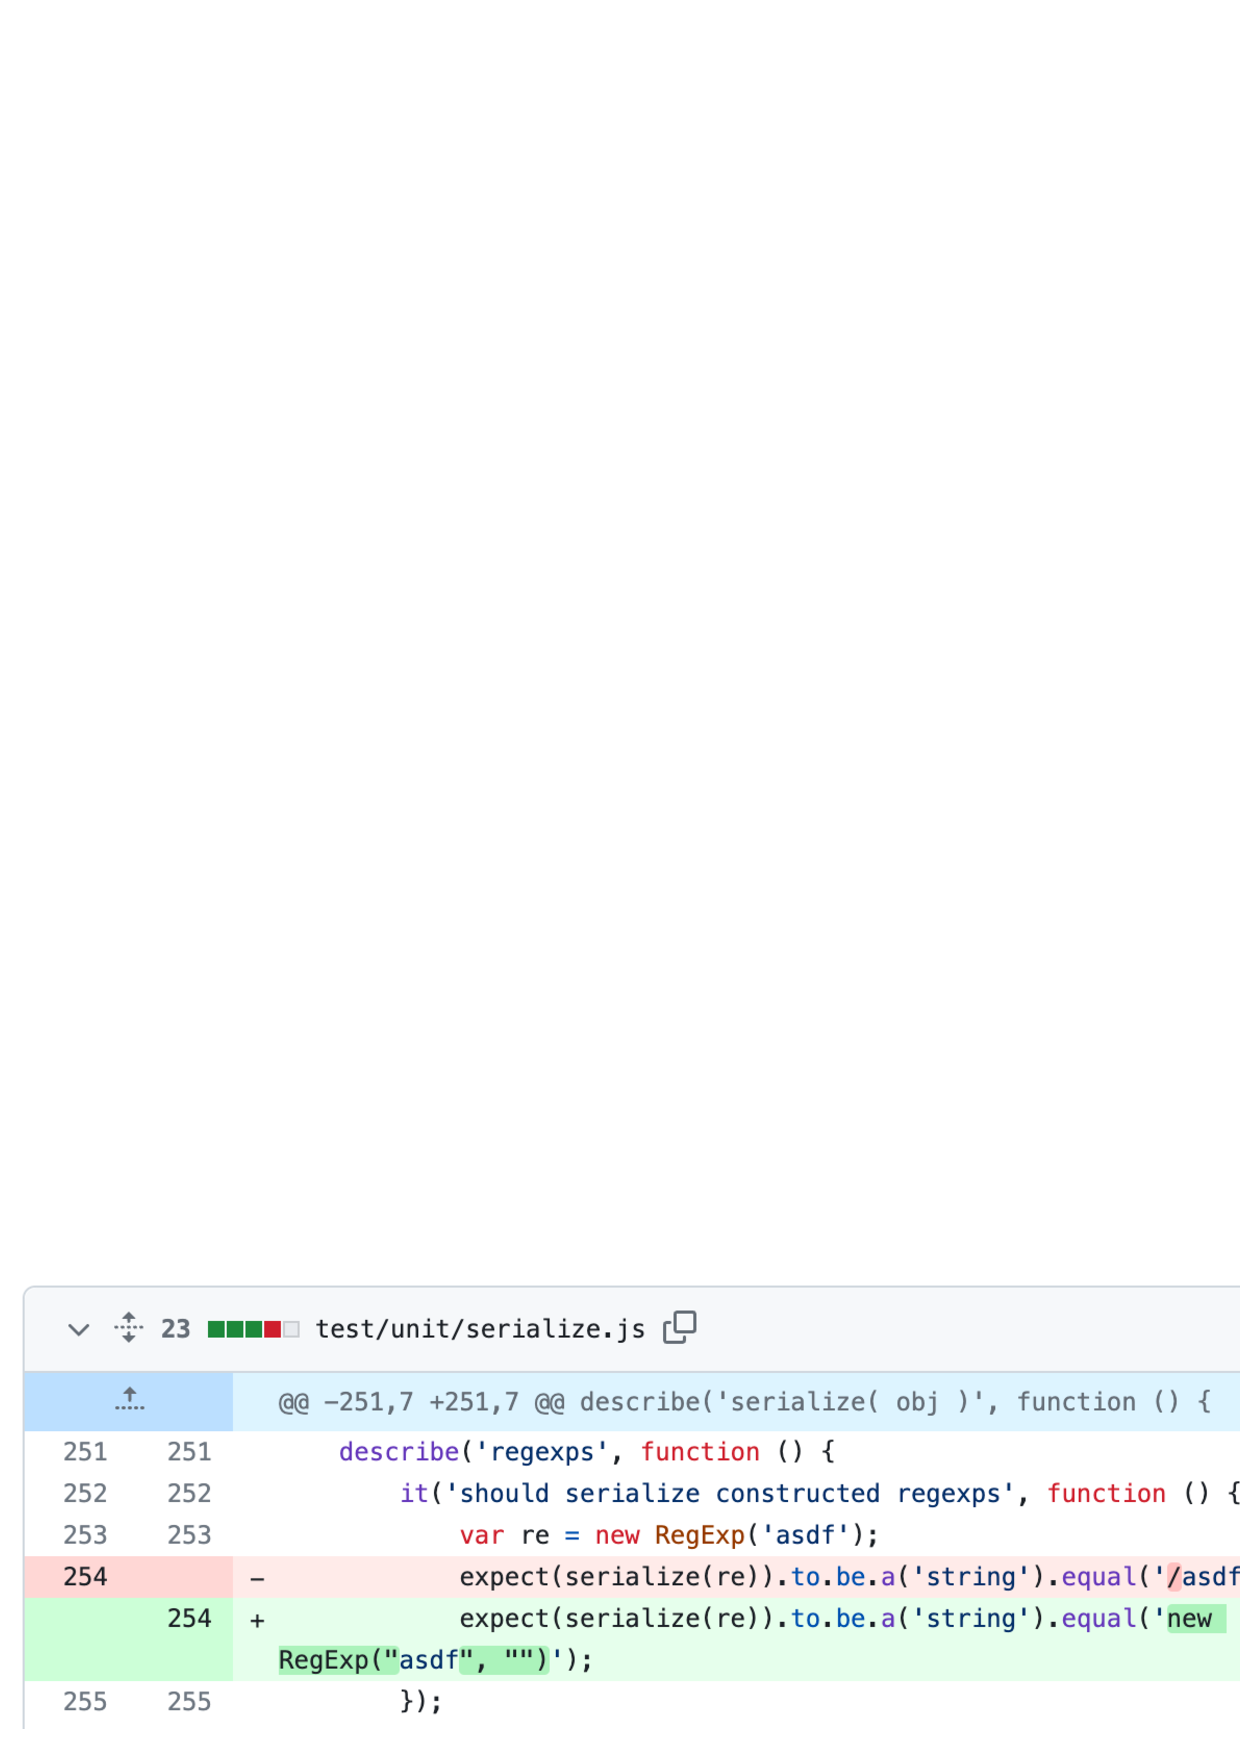
\includegraphics[width=1.0\linewidth]{IPSJjournal_maekawa_fig/rq1/serialize-javascript/index.test.pdf}
  \caption{serialize-javascriptのバージョン2.1.0から2.1.1への変更}
  \ecaption{Code changes from version 2.1.0 to 2.1.1 of serialize-javascript.}
  \label{fig:motivation}
  \vspace{-4mm}
\end{figure}
%----------------------




%クライアント開発者は,利用するライブラリのバージョンを更新する際に引き起こされるエラーを回避するために,更新後のバージョンの後方互換性を判断する必要がある.しかしながら関連研究が示すとおり,後方互換性を正確に判断することは多くの場合に困難である.

本研究では,「ライブラリの変更に伴いテストコードを変更したバージョンでは後方互換性を損失している」と仮説を立てる.テストの変更内容から後方互換性の損失を検出可能な例として,JavaScriptオブジェクトを文字列に変換する関数を提供するライブラリserialize-javascript\footnote{\url{https://github.com/yahoo/serialize-javascript/}}のバージョン2.1.0から2.1.1への更新を挙げる.
この更新ではセキュリティ修正のために,特定の入力に対する関数の出力が変更されている\footnote{\url{https://github.com/yahoo/serialize-javascript/compare/v2.1.0...v2.1.1}}.
変更内容を図\ref{fig:motivation}に示す.
図\ref{fig:motivation}上部{\verb|index.js|}はソースコード,下部の{\verb|test/unit/serialize.js|}はテストコードの変更内容である.
ソースコードの191行目で,190行目の条件に合致する特定の入力に対する関数の返り値が変更されている.この変更に伴い,テストコードの254行目の変更では,テスト対象となる関数とパラメータはそのままで,期待する返り値のみ変更している.後方互換性の損失に伴わないテストコード変更は,テストコードの実行手順の修正や,可読性向上のためのフォーマッティングなどが考えられる.ライブラリの後方互換性を判断する手段としてライブラリに付属しているテストへの変更を用いることができるが,頻繁に再利用されるライブラリに対して後方互換性を判断できるのかは明らかでない.また,テストコードの変更内容には後方互換性の損失に伴う変更と伴わない変更がある.本研究では仮説に基づき,継続的にテストが管理されているライブラリを対象として,ライブラリのテスト変更有無によって後方互換性を判断できるか否かを検証する.さらに,テストコードの変更内容をより詳細に分析することで,後方互換性の損失を正確に検出することを目指す.

%%%%%%%%%%%%%%%%%%%%%%%%%%%%%%%
\section{分析手法}
\label{sec:analyticalMethod}
%%%%%%%%%%%%%%%%%%%%%%%%%%%%%%%

本章では\ref{sec:hypothesis}章の仮説を検証するために,ライブラリのバージョン更新でテストコードにも変更が加えられた場合に,当該バージョンの適用によってクライアントが影響を受けるか否かを分析する手法を述べる.本分析は2つの手順で構成する.
図\ref{fig:overview}は,分析手法の概略図を示す.

\begin{enumerate}
\item[手順1: ] 後方互換性を損失する変更を含むライブラリバージョンの特定
\item[手順2: ] ライブラリバージョンが破壊的変更を含むか否かの検証
\end{enumerate}

本論文では,クライアントがライブラリの新しいバージョンを利用することで,クライアントテストが失敗した場合に,ライブラリの新しいバージョンに破壊的変更が加えられたと判断する.

%-------------------
\begin{figure}[t]
  \centering
  \includegraphics[width=0.95\linewidth]{IPSJjournal_maekawa_fig/overview.pdf}
  \caption{分析手法の概略図}
  \ecaption{Overview of our analysis method.}
  \label{fig:overview}
\end{figure}
%-------------------

\subsection{手順1:後方互換性を損失する変更を含むライブラリバージョンの特定}
\label{sec:step1}
%本分析では,ライブラリのバージョン更新に伴って,テストケースに変更が加えられた場合に,当該ライブラリを使用するクライアントに影響する破壊的変更を含む可能性があると考える.
%手順1では,ライブラリのバージョン更新におけるテストケースの変更有無を分析する.
%具体的には,分析対象とするライブラリからテストケースを収集し(\ref{sec:step1-1}項を参照),テストケースの変更内容に応じて破壊的変更を含む変更を加えた可能性のあるライブラリバージョンを特定する(\ref{sec:step1-2}項を参照).

\subsubsection{テストケースの収集}
\label{sec:step1-1}

本分析では,ライブラリのバージョン更新に伴って,テストケースに変更が加えられた場合に,当該バージョンには後方互換性を損失する変更を含むと考える.分析対象とするライブラリがリリースされた日付順に連続する2つのバージョンにおいて,古いバージョンを$L(X)$,新しいバージョンを$L(X+1)$とする.本研究では,ライブラリの変更に合わせて変更したテストケースが全て成功しているライブラリバージョンを対象とする.

バージョン$L(X)$と$L(X+1)$のテストファイルからテストケースを抽出する.テストケースの動作はテストケース以外のプログラムに依存している場合があるため,テストファイル中のテストケース以外のソースコードも同時に抽出する.
本研究ではJavaScript言語を対象とするため,JavaScript向けテストツールJest~\footnote{\url{https://jestjs.io/}}やMocha\footnote{\url{https://mochajs.org/}}で採用している慣習を基に,次の3つの手順でテストファイルの収集とテストケースの抽出を行う.

\begin{enumerate}
  \item テストファイル収集:ファイルパスに「test」または「spec」を含み,かつファイル名の末尾が{\verb|.js|}または{\verb|.ts|}であるファイルをテストファイルとして収集する.
  %例えば,{\verb|test.js|}や{\verb|src/index.spec.js|}などをテストファイルと判断する.
  \item テストケース抽出:テストファイル内に記述されている,関数名が\verb|it|,\verb|test|,\verb|describe|である関数呼び出しをテストケースとして抽出する.
  \item テストケースに影響を与えるソースコード抽出:抽出したテストケースをテストファイルから削除し,残った文字列をテストケースに影響を与えるソースコードとして抽出する.
\end{enumerate}

% Listing~\ref{testSample}はテストファイルの例を示す.
% 抽出規則に従い,2行目から4行目のtest関数をテストケースとして抽出する.
% その後,テストファイルからテストケースを除いて残った1行目がテストケースに影響を与えるソースコードとなる.

% \begin{figure}[h]
%     \begin{lstlisting}[caption={[upper/lower text]%
%                \begin{tabular}[t]{@{}l@{}}
%                 test/sample.js \\[1.0\normalbaselineskip]
%                \end{tabular}},frame={tb},numbers=left,label=testSample,identifierstyle={\small},xleftmargin=6mm]
% const add = require("./add");
% test("add arguments", function() {
%     expect(add(1, 2)).toBe(3);
% })
% \end{lstlisting}
% \end{figure}

\subsubsection{テストケース変更の分類と後方互換性の判断}
\label{sec:step1-2}

本手法ではテストケースの変更を,従来研究\cite{foo}と同様に変更ありが3種類(追加,削除,修正)と変更なしの合計4種類に分類し,ライブラリバージョン間の後方互換性を判断する.
% テストケースの変更内容を分類するために,テストケースとして抽出した関数について,第一引数はテストケースを一意に識別するラベル(Listing~\ref{testSample}では,{\verb|"add arguments"|})とし,第二引数をテストケースの内容を示すボディ(Listing~\ref{testSample}では,{\verb|function() { ... }|})とする.
% テストケースのラベルとボディを用いて,$L(X)$から$L(X+1)$へのバージョン更新におけるテストケースの変更を4種類に分類する.

% \begin{itemize}
% \item \textbf{変更あり(追加)} $L(X)$のテストケースに存在しなかったラベルが,$L(X+1)$に存在する.
% \item \textbf{変更あり(削除)} $L(X)$のテストケースに存在したラベルが,$L(X+1)$に存在しない.
% \item \textbf{変更あり(修正)} $L(X)$のテストケースに存在したラベルが$L(X+1)$にも存在するが,ボディが異なる.
% \item \textbf{変更なし} $L(X)$のテストケースに存在したラベルが$L(X+1)$にも存在し,ボディが同一である.
% \end{itemize}

%テストファイル中のテストケース以外の部分はテストケースに影響を与えるソースコードとして抽出する.テストケースに影響を与えるソースコードの変更はライブラリの機能全体の振る舞いの変更と考え,テスト全体として変更ありと考える.

本研究では,変更(削除または修正)を含むテストケースを1つ以上含む,またはテストケースに影響を与えるソースコードに変更(削除または修正)を含む場合,新しいバージョンに後方互換性の損失を含むと予測する.

\subsection{手順2:ライブラリ更新が破壊的変更を含むか否かの検証}
\label{sec:step2}

本分析では,ライブラリのバージョン更新に伴いライブラリに付属するテストに変更が加えられた場合に,当該ライブラリを使用する任意のクライアント$C$のテストが一つ以上失敗するか否かによって,バージョンに破壊的変更を含むか否かを検証する.

% $C$の依存ライブラリの連続する2つのバージョン$L(X)$,$L(X+1)$をそれぞれ使用したときの$C$のテスト結果と,テスト結果に基づく破壊的変更の有無の予測結果は,表\ref{fig:valid}に示す4つに分類する.

% \begin{table}[t]
%   \centering
%   \caption{ライブラリバージョン$L(X)$または$L(X+1)$を使用したクライアント$C$のテスト結果に基づく破壊的変更の有無}
%   \ecaption{hoge}
%   \label{fig:valid}
%   \scalebox{0.8}{
%   \begin{tabular}{p{2.3cm}|p{2.6cm}|p{2cm}}\hline
%     $L(X)$を使用した$C$のテスト結果 & $L(X+1)$を使用した$C$のテスト結果 & 破壊的変更 \\ \hline
%     成功 & 失敗 & あり \\ \hline
%     成功 & 成功 & 不明 \\ \hline
%     失敗 & 失敗 & 不明 \\ \hline
%     失敗 & 成功 & 不明 \\ \hline
%   \end{tabular}
%   }
% \end{table}

$L(X)$を使用した$C$のテストが成功し,$L(X+1)$を使用した$C$のテストが失敗した場合,ライブラリの変更のみによって$C$のエラーが引き起こされたと判断でき,$L(X)$から$L(X+1)$へのライブラリ更新には破壊的変更が含まれると予測する.
一方で,$L(X)$と$L(X+1)$の両方で$C$のテストが成功する場合であっても,ライブラリの変更に破壊的変更が含まれないとは限らない.また,$L(X)$を使用した$C$のテストが失敗した場合,破壊的変更有無は不明となるため分析しない.手順1と手順2を分析対象とするライブラリのバージョン更新に適用し,結果を図~\ref{fig:overview}の混同行列の4つに分類する.


%%%%%%%%%%%%%%%%%%%%%%%%%%%%%%%
\section{分析1: テストコード変更有無に基づく後方互換性損失の検出}
\label{sec:prepare}
%%%%%%%%%%%%%%%%%%%%%%%%%%%%%%%

% 分析対象とするライブラリバージョンと,後方互換性を判断するためのクライアントテストの実行結果を収集する.

\subsection{分析対象ライブラリの決定}
本研究ではMujahidらが公開するデータセット\cite{mujahid}を使用する.データセットには,GitHubリポジトリが記載されていることと,ライブラリを記述するファイル({\verb|package.json|})の変更履歴が2回以上あることを条件に,npmから収集した290,417件のJavaScriptライブラリのメタ情報が含まれている.
本研究ではこのデータセットから,3つの条件を満たす238件のライブラリを対象とする.

\begin{itemize}
\item ライブラリがテストケースに加えた変更を利用して後方互換性を判断する(\ref{sec:step1}節を参照)ため,テストコードが公開されている.
\item ライブラリの人気度合いを示すnpmスコア~\footnote{\url{https://npms.io/}}が上位500位以内であること.
\item テストを継続的に管理しているライブラリを対象とするため,各バージョンがリリースされた変更のコミットステータス\footnote{\url{https://docs.github.com/en/rest/reference/repos#statuses}}において,テスト実行時の成功率が100\%であること.
\end{itemize}

%ライブラリが持つGitHubリポジトリの各変更には,コミットステータスと呼ばれる,テストの実行結果を含むデータが紐付けられている.
%例として,serialize-javascriptは変更履歴\footnote{\url{https://github.com/yahoo/serialize-javascript/commits/2b4f837}}に登録されているコミットステータスを確認できる.%図\ref{fig:commitStatus}に示す.
%serialize-javascriptの2022年1月19日の変更では,依存ライブラリのバージョンが変更されている.
%この変更が行われた際に,同時にテストが実行され,実行結果がコミットステータスに登録されている.
%登録されている情報からテストはいずれも成功していると分かる.
%コミットステータスを使用することで,分析のためにテストを再度実行することなく,既存のテスト実行結果を利用する.

%\begin{figure}
%  \centering
%  \includegraphics[width=0.95\linewidth]{fig/commit-status.png}
%  \caption{serialize-javascriptのGitHubリポジトリに登録されているコミットステータス}
%  \label{fig:commitStatus}
%\end{figure}


\subsection{分析対象のライブラリバージョン別にクライアントテスト実行結果を収集}
\label{sec:experiment}
ライブラリバージョンの後方互換性を判断した後,後方互換性を検証するためにクライアントテスト実行結果を利用する(\ref{sec:step2}節を参照)ため,分析対象とするライブラリバージョン別にクライアントテストの実行結果を収集する.

分析対象とする238件のライブラリバージョンと,各バージョンに依存するクライアントとの組み合わせをMujahidらのデータセットから抽出した.
%抽出結果について,各ライブラリごとのクライアント数を図\ref{fig:dependencies}に示す.横軸はクライアント数ごとに並べ替えた各ライブラリ,縦軸は各ライブラリのクライアント数を示す.
238件のライブラリバージョンには平均93.6件,中央値36件のクライアントがあり,ライブラリバージョンとクライアントの組み合わせは22,271組を確認した.

クライアントにおける各ライブラリバージョンのテスト実行結果を収集するために,2つの手順を繰り返す.図\ref{fig:experimentExample}は,クライアント$C$とライブラリ$L$のバージョン$X$との組を使用し,手順を繰り返す例を示す.
\begin{enumerate}
  \item クライアントテストを実行する.テストが失敗した場合は手順を終了する.
  \item ライブラリのバージョンを一つ新しいものに更新し,(1)に戻る.新しいバージョンが無ければ手順を終了する.
\end{enumerate}
例では,手順1と手順2をそれぞれ2回繰り返した後,クライアントテスト実行が失敗することで終了し,最終的にクライアントテスト結果を3件収集する.3件のテスト結果において,$L(X+1)$を使用して成功した$C$のテストが$L(X+2)$使用時に失敗しているため,$L(X+2)$にクライアントのテスト結果を変化させる破壊的変更が含まれていたと予測する.ただし,$L(X)$を使用して成功していた$C$のテストは,$L(X+1)$使用時に成功しているが,$C$のテストが不十分なことも考えられるため,$L(X+1)$の後方互換性は不明とする.





%\begin{figure}
%  \centering
%  \includegraphics[width=0.6\linewidth]{IPSJjournal_maekawa_fig/dependencies.pdf}
%  \caption{分析対象ライブラリ(238件)ごとのクライアント数の分布(1≦n≦238)}
%  \label{fig:dependencies}
%\end{figure}

%---------------------
\begin{figure}[t]
  \centering
  \includegraphics[width=1\linewidth]{IPSJjournal_maekawa_fig/experiment-example1.pdf}
  \caption{クライアントテスト実行結果の収集方法}
  \ecaption{Collecting approach of client test results.}
  \label{fig:experimentExample}
  \vspace{-4mm}
\end{figure}
%---------------------

クライアントテストが失敗したライブラリ以降にリリースされたバージョンは,同じクライアントテストで成功することが見込めないため分析対象としない.
%上記手順によって71,342件のクライアントテストを実行し,結果を収集した.


\subsection{テスト結果に基づいて分析対象ライブラリバージョンを決定}

\ref{sec:experiment}節で収集した結果に基づいて,後方互換性を判断するライブラリバージョンを決定し,後方互換性を検証するためのクライアントテストの実行結果を次の3つの手順で集計する.
\begin{enumerate}
  \item \ref{sec:experiment}節で,テスト結果を1件しか収集できず,$L(X)$と$L(X+1)$の組ができないものを除く.
  \item 全てのクライアントテストの実行結果について,$L(X)$と$L(X+1)$,$L(X+1)$と$L(X+2)$のようにバージョン更新ごとの組を作る.
  \item 異なるクライアントが同じライブラリバージョンの組を使用した場合はクライアントテストの実行結果を統合する.
\end{enumerate}
集計の結果,ライブラリバージョンとクライアントの組み合わせ1,955組を分析対象とする.

\subsection{分析結果}

% \subsection{概要}
% 本章では,後方互換性の損失を含むライブラリ更新に伴うテストコードの変更内容を分析し,後方互換性の損失を検出する手掛かりとなるテストコードの変更内容を明らかにする.具体的には,各ライブラリバージョンに対して,後方互換性の有無とテストコードの変更内容を目視で調査する.

表\ref{fig:result1}は,ライブラリバージョンとクライアントの組み合わせ1,955組に対して\ref{sec:analyticalMethod}章で述べた分析手法を適用した結果を示す.
本手法により,後方互換性を損失しているライブラリバージョン223件中140件(適合率:約63\%)を正しく予測できた.223件中83件(約37\%)を目視で確認したところ,破壊的変更が行われた箇所に対応するテストが存在しないため誤って後方互換性ありと予測している事例を確認した.このような誤検出への対策として,テストを自動生成することで不足分を補填することが考えられる.

また,後方互換性なしと予測したライブラリバージョン905件中140件(再現率:約15\%)のみを正しく予測できた.905件中765件(約85\%)が不明に分類された原因として,クライアントが後方互換性を損失している関数を使用していない,クライアントのテストケースが不十分であることが示唆される.

本手法は,ライブラリバージョンのテストケースの変更方法のみに着目し,後方互換性の損失の予測を試みているが,テストケースの変更内容によってはリファクタリングのような後方互換性の損失に関係しない変更も存在すると考える.\ref{sec:contentAnalysis}章では,後方互換性の損失に影響するテストケースの変更内容を調査する.

%実際にテストを調査した内容については,\ref{sec:discussion}章で言及する.

% \begin{table}[t]
%   \centering
%   \caption{分析結果}
%   \label{fig:result}
%   \scalebox{1.0}{
%   \begin{tabular}{l|r|r|r}\hline\hline
%      & \multicolumn{2}{c|}{テスト変更}  & \multirow{2}{*}{合計} \\ \cline{2-3}
%      & あり & なし &  \\ \hline
%     クライアントテストが一つ以上失敗 & 183 & 85 & 268 \\ \hline
%     クライアントテストが全て成功 & 856 & 987 & 1,843 \\ \hline
%     合計 & 1,039 & 1,072 & 2,111 \\ \hline
%   \end{tabular}
%   }
%   %\vspace{-5mm}
% \end{table}

%------------------
\begin{table}[t]
  \centering
  \caption{テストコード変更有無に基づく後方互換性損失の検出結果}
  \ecaption{Detection results of backward compatibility loss due to test code changes.}
  \label{fig:result1}
  \scalebox{0.9}{
  \begin{tabular}{l|r|r|r}\hline\hline
     & \multicolumn{2}{c|}{後方互換性}  & \multirow{2}{*}{合計} \\ \cline{2-3}
     & なし & 不明 &  \\ \hline
    後方互換性なしと予測 & 140 & 765 & 905 \\ \hline
    後方互換性ありと予測 & 83 & 967 & 1,050 \\ \hline
    合計 & 223 & 1,732 & 1,955 \\ \hline
  \end{tabular}
  }
  \vspace{-5mm}
\end{table}
%------------------

% \subsection{分析結果}\label{seq:rq1-result}

% \subsubsection{後方互換性の有無の判定}\label{subsec:kouhougokanseinohantei}
% 後方互換性の有無の判定には,従来手法と同様,Mujahidらの手法を使用する.Mujahidらは,ライブラリの後方互換性の損失をクライアントテストを実行することで検出する手法を提案した\cite{mujahid}.後方互換性を損失する変更を加えられたライブラリバージョンでは,その影響を受けるクライアントテストの結果が更新前後で成功から失敗に変化することを手法の根拠としている.本分析も同様に,対象ライブラリのクライアントに対し,次の手順で後方互換性の有無を判定する.

% \begin{enumerate}
%   \item クライアントテストを実行する.テストが失敗した場合は分析対象外とする.
%   \item ライブラリのバージョンを新しいものに更新し,クライアントテストを実行する.クライアントテストが失敗した場合,後方互換性を損失したと判定する.
% \end{enumerate}

%%%%%%%%%%%%%%%%%%%%%%
\section{テストコード変更内容の分析}\label{sec:contentAnalysis}
%%%%%%%%%%%%%%%%%%%%%%

本章では,後方互換性の損失を検出する手掛かりとなるテストコードの変更内容を明らかにするために,後方互換性の有無とテストコードの変更内容を著者らが目視で調査する.分析対象とするテストコードの変更内容として,本研究では後方互換性の損失に関係することを示唆するテストコードの構成要素5項目(変更内容10種類),および後方互換性の損失に関係しないと示唆する変更内容1種類(リファクタリング),の合計11種類の変更内容を分析する.

\begin{itemize}
  \item テストスイートの変更2種類(追加,削除)
  \item テストケースの変更2種類(追加,削除)
  \item アサーションの変更4種類(追加,削除,入力値の変更,期待値の変更)
  \item テストの前提条件の変更1種類
  \item テストフィクスチャの変更1種類
  \item リファクタリングのための変更1種類  
\end{itemize}
\vspace{-4mm}

% テストコード変更内容を目視分類するために,テストコードの構成要素をまとめる.本研究では,プログラムのテストの中でも単体テストを対象とする.単体テストとは,関数やクラスなどのプログラムを構成する単位(ユニット)が開発者の期待通りに動作するかを検証するテスト手法である.単体テストを実施する際は,テスト対象ユニットに対応するテストスイートを用意する必要がある.テストスイートとは,テストの目的や条件が似ているテストケースの集合を指す.テストケースは,テスト項目の最小単位であり,テスト対象への入力と期待される結果(期待値)の組み合わせで構成する.入力値と期待値を受け取ってプログラムが正しく動作しているか検証する仕組みをアサーションと呼ぶ.

% \begin{figure}[t]
% \begin{lstlisting}[caption=Calculator.js, label=Calculator.js]
% class Calculator {
%   add(a, b) {
%     return a + b;
%   }
% }
% \end{lstlisting}
% \end{figure}

% \begin{figure}[t]
% \begin{lstlisting}[caption=Calculator.test.js, label=Calculator.test.js]
% import { Calculator } from './Calculator';

% describe('Calculator', () => {
%   let calculator;

%   beforeEach(() => {
%     calculator = new Calculator();
%   });

%   test('should add two positive numbers', () => {
%     if (calculator) {
%       expect(calculator.add(1, 1)).toBe(2);
%     }
%   });
% });
% \end{lstlisting}
% \end{figure}

% Program~\ref{Calculator.js},Program~\ref{Calculator.test.js}は,JavaScriptにおけるテストコードの例を示す.Program~\ref{Calculator.js}は,テスト対象となるクラス{\verb|Calculator|}が定義されている.このクラスに含まれるメソッド{\verb|add()|}は,2つの引数を受け取り足し合わせた値を返す.Program~\ref{Calculator.test.js}は,{\verb|Calculator|}クラスを単体テストによって検証するファイルで,JavaScript向けテストフレームワークJest\footnote{\url{https://jestjs.io/}}を使用して記述している.

% Program~\ref{Calculator.test.js}は,3行目の{\verb|describe|}関数でテストスイートを宣言し,10行目の{\verb|test|}関数により1つのテストケースを定義している.テストスイートやテストケースは,何を検証するかが記述されるラベルと,動作を検証するテスト用関数を引数に取る.6行目から7行目の{\verb|beforeEach|}関数で,テストフィクスチャと呼ばれる,テストデータの初期化などのテストの事前条件を定義する.例では,{\verb|Calculator|}クラスをインスタンス化している.10行目から12行目で定義されるテストケースは,11行目で{\verb|if|}文によりテストの前提条件を記述し,12行目のアサーションで{\verb|Calculator.add()|}に対し1と1を入力したときの動作を検証している.この場合,期待する結果は2であるため,{\verb|toBe|}節で結果が2となる.以上より,本研究ではJavaScript言語のテストコードの構成要素として次の5件を定義する.

% \begin{itemize}
%   \setlength{\itemsep}{0cm}
%   \item テストスイート
%   \item テストケース
%   \item アサーション(入力値,期待値を含む)
%   \item 前提条件
%   \item テストフィクスチャ
% \end{itemize}

% テストコードの変更内容として,テストコードの構成要素それぞれを追加,変更,削除する変更内容が考えられる.アサーションの期待値,入力値はテストコードの最小単位であるため変更のみ考慮し,前提条件については追加,削除も前提条件が変更されたと考えられるため変更のみを考慮する.テストスイート・テストケースのラベルの変更,テストフレームワークの変更,可読性向上のためのフォーマッティングなどテストコードの振る舞いに関わらない変更については,リファクタリングとする.以上を踏まえ,本研究ではテストコードの変更内容として次の11件を考慮する.

% \begin{itemize}
%   \setlength{\itemsep}{0cm}
%   \item テストスイートの追加
%   \item テストスイートの削除
%   \item テストケースの追加
%   \item テストケースの削除
%   \item アサーションの追加
%   \item アサーションの削除
%   \item アサーションの入力値の変更
%   \item アサーションの期待値の変更
%   \item テストの前提条件の変更
%   \item テストフィクスチャの変更
%   \item リファクタリング
% \end{itemize}


\subsection{データセット}\label{rq1:datasets}

\ref{sec:prepare}章で分析対象とした1,955件のライブラリバージョンからライブラリテストに変更があるライブラリバージョン1,027件を抽出し,ランダムサンプリング(信頼区間95\%,信頼度5\%)した280件を目視調査することでテスト変更内容ごとの後方互換性を維持,または損失したバージョン数を明らかにする.

% データセットとして,従来研究\cite{matsuda}で収集されたライブラリバージョン群を使用する.従来研究では,ライブラリの人気度を示すnpmスコア~\footnote{\url{https://npms.io}}が上位500件以内で,各バージョンのコミットにおけるテスト実行時の成功率が100%であることを条件にnpm\footnote{\url{https://www.npmjs.com/}}から2,111件のライブラリバージョンを収集した.本調査では,このデータセットから,ライブラリテストに変更があるライブラリバージョン1,027件を抽出し,95%の信頼区間でサンプリングした280件を対象とする.分析対象とするライブラリと,各ライブラリのいずれかに依存するクライアントとの組み合わせは,Mujahidらのデータセットから抽出した.

%--------------------
\begin{figure}[t]
  \centering
  \includegraphics[width=1.0\linewidth]{IPSJjournal_maekawa_fig/barh-test-pattern.pdf}
  \caption{テスト変更内容別の後方互換性の損失率}
  \ecaption{Rate of backward compatibility loss each test code change type.}
  \label{fig:test_pattern}
  \vspace{-4mm}
\end{figure}
%--------------------

\subsection{分析結果}

図\ref{fig:test_pattern}は,テスト変更内容ごとの後方互換性の有無を積み上げ横棒グラフで示す.横軸は各テストコード変更のライブラリバージョン数,縦軸は各ライブラリバージョンにおけるテストコード変更内容である.破線より上の変更内容は分析1の手法で後方互換性を維持すると判定し,破線より下の変更内容は後方互換性を損失すると判定している.

ライブラリバージョンにおいてテスト変更内容は,テストコード(テストスイート,テストケース)の追加,テストコード(テストスイート,テストケース)の削除,テストコードの変更(アサーションの追加,アサーションの入力値/期待値の変更,テストフィクスチャの変更)するときに後方互換性の損失していることが多い.これらについては,\ref{subsec:add-test}項から\ref{subsec:change-test}項においてそれぞれ事例を挙げながら説明する.これら以外に,後方互換性を損失するライブラリ更新に伴って,ライブラリの更新とは無関係にテストがリファクタリングされることも確認したが,本研究ではライブラリの更新に関係するテストの変更のみに着目する.

% \subsubsection{従来手法で後方互換性を維持すると判定するテスト変更内容}
% 従来手法で後方互換性を維持すると判定するテスト変更内容は,テストスイートの追加,テストケースの追加である.これらは,後方互換性を維持するライブラリ更新に伴う場合が多いため,従来手法で誤検出となる主な原因ではない.ただし,後方互換性を損失するライブラリ更新に伴ってテストスイートやテストケースを追加する場合もある.具体的な例は\ref{subsec:add-test}項で述べる.

% \subsubsection{従来手法で後方互換性を損失すると判定するテスト変更内容}
% 従来手法で後方互換性を損失すると判定するテスト変更内容は,テストスイートの削除,テストケースの削除,アサーションの追加,アサーションの削除,アサーションの入力値の変更,アサーションの期待値の変更,前提条件の変更,テストフィクスチャの変更,リファクタリングである.このうち,リファクタリングは後方互換性を維持するライブラリ更新に伴う場合が多く,件数も多いため従来手法で誤検出となる主な原因であるとわかる.一方,リファクタリングが後方互換性を損失するライブラリ更新に伴う場合もある.これは,後方互換性を損失するライブラリ更新に伴って,無関係にテストがリファクタリングされることがあることを示す.テストスイートの削除,テストケースの削除は,後方互換性を損失するライブラリ更新に伴う場合が多いため,従来手法で誤検出となる主な原因ではない.ただし,後方互換性を維持するライブラリ更新に伴ってテストスイートやテストケースを削除する場合もある.具体的な例は\ref{subsec:delete-test}項で述べる.アサーションの追加,アサーションの入力値の変更,アサーションの期待値の変更,前提条件の変更は,後方互換性を維持するライブラリ更新に伴う場合が多く,従来手法で誤検出となる主な原因である.ただし,後方互換性を損失するライブラリ更新に伴って,アサーションを追加したり,アサーションの入力値,アサーションの期待値を変更する場合もある.具体的な例は,それぞれ\ref{subsec:add-test}項,\ref{subsec:change-test}項で述べる.テストフィクスチャの変更は,テストデータの初期化や事前条件を定義する性質上,変更時のテストコードの影響範囲が広く,後方互換性の損失との関係を分析することが困難であるため,本研究では対象としない.

% 続く\ref{rq2:kousatu}節では,テスト変更内容をテストコード追加,テストコード削除,テストコード変更に分けて,後方互換性を損失するライブラリ更新に伴うテストコード変更内容,伴わないテストコード変更内容をそれぞれ例を挙げる.

\subsubsection{テストコード追加}\label{subsec:add-test}

% %-----------
% \begin{figure}[t]
%   \centering
%   \includegraphics[width=1.0\linewidth]{IPSJjournal_maekawa_fig/rq1/set-map/map.pdf}
%   \caption{serialize-javascriptのバージョン1.6.1から1.7.0のソースコード変更差分}
%   \label{fig:rq1.insert-test-src}

%   \centering
%   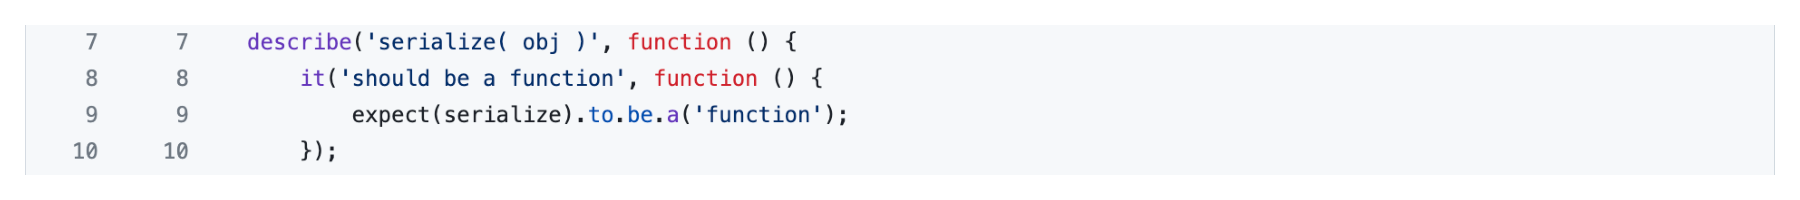
\includegraphics[width=1.0\linewidth]{IPSJjournal_maekawa_fig/rq1/set-map/map.test.1.eps}
%   \includegraphics[width=1.0\linewidth]{IPSJjournal_maekawa_fig/rq1/set-map/map.test.2.eps}
%   \caption{serialize-javascriptのバージョン1.6.1から1.7.0のテストコード変更差分}
%   \label{fig:rq1.insert-test-test}
% \end{figure}
% %-----------

テストコード追加は,テスト対象となるAPIの追加など後方互換性を維持するライブラリ更新に伴う場合が多い.ただし,後方互換性を損失するライブラリ更新に伴ってテストコードが追加されることがある.JavaScriptオブジェクトを文字列に変換するAPIを提供するライブラリserialize-javascriptのバージョン1.6.1から1.7.0へのマイナーアップデートでは,関数{\verb|serialize|}に,JavaScriptの{\verb|Map|}型のデータを文字列に変換する機能が追加された(ファイル{\verb|index.js|},155行目から157行目\footnote{\url{https://github.com/yahoo/serialize- javascript/compare/v1.6.1...v1.7.0}}).この変更に伴って,関数{\verb|serialize|}に関するテストスイートに,新しく{\verb|Map|}型のデータが正確に文字列に変換されるかを検証するテストスイートが追加された(ファイル{\verb|test/unit/serialize.js|,201行目から220行目\footnotemark[13]).バージョン1.6.1では,関数{\verb|serialize|}は{\verb|Map|}型の入力を文字列に変換する機能を持っていないため,文字列に変換されないことに依存しているクライアントはバージョン更新の際に返り値が新しくなったことによる影響を受ける.このようなAPIの機能拡張による後方互換性の損失は,既存のテストスイート内にテストコードが追加されるという特徴があるため,既存のテストスイート内にテストスイート,テストケース,アサーションが追加された場合,ライブラリの後方互換性を損失したと判断できると考えられる.

\subsubsection{テストコード削除}\label{subsec:delete-test}

% %-----------
% \begin{figure}[t]
%   \centering
%   \includegraphics[width=1.0\linewidth]{IPSJjournal_maekawa_fig/rq1/uuid/randomBytes2.pdf}
%   \includegraphics[width=1.0\linewidth]{IPSJjournal_maekawa_fig/rq1/uuid/randomByte.pdf}
%   \caption{uid-safeのバージョン2.0.0から2.1.0のソースコード変更差分}
%   \label{fig:rq1.delete-test-src}

%   \centering
%   \includegraphics[width=1.0\linewidth]{IPSJjournal_maekawa_fig/rq1/uuid/randomByte-test.pdf}
%   \caption{uid-safeのバージョン2.0.0から2.1.0のテストコード変更差分}
%   \label{fig:rq1.delete-test-test}
% \end{figure}
% %-----------

テストコード削除は,テスト対象となるAPIの削除など後方互換性を損失するライブラリ更新に伴う場合が多い.ただし,後方互換性を維持するライブラリ更新に伴ってテストコードが削除されることがある.暗号化されたUIDを生成するAPIを提供するライブラリuid-safeのバージョン2.0.0から2.1.0へのマイナーアップデートでは,セキュリティ上の問題から,ランダムなバイト列を生成する関数{\verb|randomBytes|}を削除し,同等のモジュールに置き換えている(ファイル\verb|index.js|,16行目\footnote{\url{https://github.com/crypto-utils/uid-safe/compare/2.0.0...2.1.0}}).この変更に伴って,関数{\verb|randomBytes|}の動作を検証するテストスイートが削除されている(ファイル\verb|test/test.js|,40行目から54行目\footnotemark[14]).モジュールの置き換え前後で関数{\verb|randomBytes|}の振る舞いが全く同じ場合,後方互換性を維持する.本研究では,\ref{sec:prepare}章で述べた通り,後方互換性の有無の判定にクライアントテストを利用している.このようなモジュールに置き換える例では,振る舞いの変化が限定的になるため,クライアントテストが捉えられず後方互換性を維持したと誤検出することが考えられる.誤検出を防ぐには実際に影響を受けるクライアントの特定が必要になるが,容易ではない\cite{detecting-locations-in-js}.従って,本研究ではテストコード削除の検出は行うが,影響するクライアントの特定,およびクライアントテストの調査は今後の課題とする.

\subsubsection{テストコード変更}\label{subsec:change-test}

% %-----------
% \begin{figure}[t]
%   \centering
%   \includegraphics[width=1.0\linewidth]{IPSJjournal_maekawa_fig/rq1/rejection/rejection-test.pdf}
%   \caption{loud-regectionのバージョン1.2.1から1.3.0のテストコード変更差分}
%   \label{fig:rq1.change-test-rejection-test}
% \end{figure}
% %-----------

% \begin{figure}[t]
%   \centering
%   \includegraphics[width=1.0\linewidth]{IPSJjournal_maekawa_fig/rq1/rgb/rgb-src.pdf}
%   \includegraphics[width=1.0\linewidth]{IPSJjournal_maekawa_fig/rq1/rgb/rgb-src-1.pdf}
%   \caption{color-stringのバージョン0.4.0から1.0.0のソースコード変更差分}
%   \label{fig:rq1.change-test-input-src}


%   \centering
%   \includegraphics[width=1.0\linewidth]{IPSJjournal_maekawa_fig/rq1/rgb/rgb-test.pdf}
%   \caption{color-stringのバージョン0.4.0から1.0.0のテストコード変更差分}
%   \label{fig:rq1.change-test-input-test}
% \end{figure}
% %-----------


%アサーションの入力値,期待値の変更やリファクタリングなどのテストコード変更は,ライブラリの更新とは無関係に行われることもある.ライブラリの更新とは無関係にアサーションの入力値,期待値が変更される例として,非同期処理のエラー内容を追跡するAPIを提供するライブラリloud-regectionのバージョン1.2.1から1.3.0へのマイナーアップデート\footnote{\url{https://github.com/sindresorhus/loud-rejection/compare/v1.2.1...v1.3.0}}では,アサーションメソッドを{\verb|true()|}から{\verb|regex()|}に変更しており,アサーションの入力値と期待値が同時に変更されている.ただし,テストコードの振る舞いは変わっておらず,ソースコードの変更とは無関係のテストコード変更である(ファイル\verb|test.js|,73行目).一方,\todo{X節で説明した図Xのように}後方互換性を損失するライブラリ更新に伴って,アサーションの入力値,期待値が変更されることがある.
%アサーションの期待値が変更される例は,\ref{sec:key-idea}節で示したので割愛する.

後方互換性を損失するライブラリ更新に伴って,アサーションの入力値,期待値が変更されることがある.CSSの色文字列を解析するAPIを提供するライブラリcolor-stringのバージョン0.4.0から1.0.0のメジャーアップデートでは,関数{\verb|rgbString|}を{\verb|to.rgb|}に置き換えている(ファイル\verb|color-string.js|の154行目から160行目を削除,ファイル\verb|index.js|の129行目から135行目を追加\footnote{\url{https://github.com/Qix-/color-string/compare/0.4.0...1.0.0}}).この変更に伴って,関数{\verb|rgbString|}に関するアサーションの入力値が変更されている.ファイル\verb|test/basic.js|のテストケース\footnotemark[15]は,変更前68行目から74行目と変更後62行目から68行目は1行ずつ対応しており,アサーションの{\verb|equal|}関数の第一引数の入力値が変更され,第二引数の期待値は変更されていない.従って,APIの入出力形式の変更による後方互換性の損失は,アサーションの期待値もしくは入力値のいずれか一方だけ変更されるという特徴があるため,アサーションの入力値と期待値のいずれか一方が変更された場合,後方互換性を損失したと判断できると考えられる.

\vspace{-2mm}
\subsection{まとめ}
本章では,後方互換性を損失するライブラリ更新に伴ってどのようなテストコード変更が行われているかを分析し,後方互換性の損失を検出する手掛かりとなるテストコード変更内容を明らかにした.結果「既存のテストスイート内でのテストコード追加」「テストコード削除」「アサーションの入力値と期待値のいずれか一方の変更」の3つが後方互換性の損失を検出する手掛かりになる,機械的に検出可能なテストコード変更であると考える.

\vspace{-2mm}
%%%%%%%%%%%%%%%%%%%%%%%%%%%%%%%
\section{分析2: テストコード変更内容に基づく後方互換性損失の検出}\label{chap:rq2}
%%%%%%%%%%%%%%%%%%%%%%%%%%%%%%%

\ref{sec:contentAnalysis}章において,後方互換性を損失するライブラリバージョンでは,テストコードの追加,削除,変更が後方互換性の損失を検出する手掛かりになることを明らかにした.本章では,これらのテストコードの変更を自動検出するツールを開発し,後方互換性の損失の検出精度を評価する.
`
% \subsection{ルール構築}\label{sec:rq2.teian}

% 本研究が提案する自動検出ツールは,入力を全てのソースファイル,出力を後方互換性の有無の予測とする.まず,入力として与えられた変更前後の全てのソースファイルから,変更されていないファイルを除外し,テストコードが記述されたファイルを抽出する.従来研究\cite{matsuda}では,テストコードが記述されたファイルの条件を,ファイルパスに{\verb|test|}または{\verb|spec|}を含み,ファイル名の末尾が{\verb|.js|}または{\verb|.ts|}であるファイルとする.本研究ではこの条件に加え,ファイル名の末尾が{\verb|.d.ts|}でないファイルを条件とする.ファイル名の末尾が{\verb|.d.ts|}であるファイルは型定義ファイルであり本研究では除外する.次に,抽出したソースファイルにおける,プログラムの変更箇所とその変更方法を\ref{subsec:rq2.astseisei}項の方法で特定する.最後に,プログラムの変更箇所とその変更方法が\ref{subsec:rq2.jouken}項で述べる3つの条件に1つでも一致すれば,後方互換性が損失していると判定し,いずれにも一致しなければ後方互換性を維持していると判定する.

\subsection{ソースコードの変更箇所と変更方法の特定}\label{subsec:rq2.astseisei}
本研究では,ライブラリバージョンにおけるテストコードの変更箇所,および変更方法を特定する.テストコードが記述されたファイルの特定は,\ref{sec:analyticalMethod}章と同様に,ファイルパスに{\verb|test|}または{\verb|spec|}を含み,ファイル名の末尾が{\verb|.js|}または{\verb|.ts|}であるファイルとする.また,ファイル名の末尾が{\verb|.d.ts|}であるファイルは型定義ファイルであるため本研究では対象外とする.

ソースコードの変更箇所と変更方法の特定のために,コミット間の差分解析ツールGumTree\cite{gumtree}を使用する.GumTreeはソースコードの構造を表す抽象構文木(以降,AST)に基づく差分解析ツールであり,構造単位で比較するため,行単位の差分解析に比べて細粒度な変更箇所の特定が可能である.GumTreeは,他の抽象構文木に基づく差分解析ツール\cite{diff-1}\cite{diff-2}\cite{diff-3}と比べて精度が高く,JavaやJavaScriptなど複数のプログラミング言語に対応している.GumTreeは,変更前後のソースファイルまたはASTを受け取ると,それらを比較してASTのノード単位の編集操作を出力する.検出できる編集操作は,「削除」「挿入」「移動」「変更」である.ただし,GumTreeはファイル単位の差分しか検出することができず,ファイルを横断するソースコードの移動は「削除と挿入」として検出されてしまうため,藤本ら\cite{gumtreenoyatu}が提案するソースコードごとに生成されるASTの結合により問題を解決する.

% \begin{enumerate}
%   \setlength{\itemsep}{0cm}
%   \item 変更のある各ファイルごとにASTを生成する
%   \item 根となるノードを1つ作成する
%   \item 各ファイルごとに生成したASTを子ノードとして加えていく
%   \item 1から3を変更前後で実施し,2つASTを生成する
%   \item 変更前後で生成された2つのASTをGumTreeに入力して出力を得る
% \end{enumerate}

% この方法により,バージョン間のテストコード変更に対して,プログラムの変更箇所(ノード)と,「削除」「挿入」「移動」「変更」の4つの変更方法をファイルを横断する移動操作も含めて特定することができる.

\vspace{-2mm}
\subsection{後方互換性を損失したバージョンの判定条件}\label{subsec:rq2.jouken}
\ref{sec:contentAnalysis}章で述べた,テストコードの追加,テストコードの削除,テストコードの変更を自動で検出するために,それぞれ条件を定義する.

テストコードの追加,テストコードの削除では,\ref{sec:contentAnalysis}章で述べたように,テストファイル内で記述されている関数名が{\verb|it|},{\verb|test|},{\verb|describe|}をテストケースとし,いずれかの関数呼び出しにおいて第一引数が文字列,第二引数が関数であるものをテストスイートまたはテストケースと定義する.

% まず,「既存のテストスイート内でのテストコード追加」「テストコード削除」を判定するために,テストコードを定義する.従来研究\cite{matsuda}では,テストファイル内に記述されている,関数名が{\verb|it|}または{\verb|test|}である関数呼び出しをテストケースとしている.本研究では,テストスイートの追加・削除を含めるため,慣習的にテストスイートの宣言として使われる関数名{\verb|describe|}を加え,{\verb|it|}または{\verb|test|}または{\verb|describe|}のいずれかの関数呼び出しで,第一引数が文字列,第二引数が関数であるものをテストスイートまたはテストケースと定義する.

テストコードの変更においては,JavaScript言語のアサーションの記述方法はフレームワークによって異なるため,State of JavaScript 2022\footnote{\url{https://2022.stateofjs.com/}}で紹介されている主要なテストフレームワーク13件のうち,単体テストで使われるフレームワーク5件(Jest\footnote{\url{https://jestjs.io/}},Mocha\footnote{\url{https://mochajs.org/}},AVA\footnote{\url{https://github.com/avajs/ava}},Jasmine\footnote{\url{https://jasmine.github.io/}},Vitest\footnote{\url{https://vitest.dev/}})で記述されたテストコードを対象とする.Mochaは複数のアサーションの記述スタイルを利用できるため,Mochaで使用可能なアサーションのスタイルについても対象とする.テストフレームワーク毎のアサーションの書き方は,2つに大別できる.例をListing \ref{bdd.test.js},Listing \ref{tdd.test.js}で示す.

% 次に,「アサーションの入力値と期待値のいずれか一方の変更」を判定するために,アサーションの入力値と期待値を定義する.JavaScript言語では,アサーションの書き方はフレームワークによって異なる.本手法では,State of JavaScript 2022\footnote{\url{https://2022.stateofjs.com/}}で紹介されている主要なテストフレームワーク13件のうち,単体テストで使われるフレームワーク5件(Jest\footnote{\url{https://jestjs.io/}},Mocha\footnote{\url{https://mochajs.org/}},AVA\footnote{\url{https://github.com/avajs/ava}},Jasmine\footnote{\url{https://jasmine.github.io/}},Vitest\footnote{\url{https://vitest.dev/}})を対象とする.Mochaは複数のアサーションの記述スタイルを利用できるため,Mochaで使用可能なアサーションのスタイルについても対象とする.テストフレームワーク毎のアサーションの書き方は,大きく2つに大別できる.例をProgram\ref{bdd.test.js},Program\ref{tdd.test.js}で示す.

\begin{figure}[t]
\begin{lstlisting}[caption=アサーション例1, label=bdd.test.js]
expect(calculator.add(1, 1)).to.be.a('number').equal(2);
expect(calculator.add(1, 1), 'to be', 2);
calculator.add(1, 1).should.be.a('number').equal(2);
\end{lstlisting}

\vspace{-3mm}

\begin{lstlisting}[caption=アサーション例2, label=tdd.test.js]
assert.equal(calculator.add(1, 1), 2);
t.is(calculator.add(1, 1), 2);  
t.true(calculator.add(1, 1) === 2);
\end{lstlisting}
\vspace{-3mm}
\end{figure}



Listing \ref{bdd.test.js}は,自然言語に似た構文を使用してテストを記述する記述形式で,Jest,Mocha,Jasmine,Vitestで使用される.その中でも,1行目のように,{\verb|expect|}関数にメソッドチェーンで振る舞いを記述する形式,2行目のように{\verb|expect|}関数の引数にそのまま振る舞いを記述する形式,3行目のように入力値に{\verb|should|}プロパティを追加して振る舞いを記述する形式がある.1,2行目の形式に対しては,{\verb|expect|}関数の第一引数を入力値,それ以降を期待値として扱い,3行目の形式に対しては,{\verb|should|}プロパティ以前を入力値,それ以降を期待値として扱う.


Listing \ref{tdd.test.js}は,Node.js\footnote{\url{https://nodejs.org/en}}標準の{\verb|assert|}文がメインの記述形式で,AVA,Mochaで使用される.その中でも,1行目や2行目のように,第一引数に入力値,第二引数に期待値を取る形式と,3行目のように入力だけを引数に取る形式がある.この記述形式に対しては,{\verb|assert|},{\verb|t|},{\verb|test|}をキーとして,アサーションメソッドの第一引数を入力,第二引数を期待値として扱う.3行目のように引数が1つの場合は,引数を入力,アサーションメソッド名を期待値とする.

これらのテストコードを対象にテストコードの追加,テストコードの削除,テストコードの変更をそれぞれ検出する3つの条件を定める.

\begin{description}
  \item[\textbf{テストコードの追加}]:GumTreeで「挿入」と判定された変更箇所がテストコードまたはアサーションであり,かつ既存のテストコード内で追加されていること
  \item[\textbf{テストコードの削除}]:GumTreeで「削除」と判定された変更箇所がテストコードであること
  \item[\textbf{テストコードの変更}]:GumTreeで「変更」と判定された変更箇所がアサーションの入力値もしくは期待値であり,同一アサーションの入力値もしくは期待値がGumTreeで「変更」と判定されていないこと
\end{description}

ライブラリバージョンに含まれるテストコード変更内容が,以上3つの条件に1つでも当てはまれば,ライブラリバージョンは後方互換性を損失したと判定し,1つも当てはまらなければライブラリバージョンは後方互換性を維持したと判定する.

\vspace{-2mm}
\subsection{分析結果}

% データセットは,\ref{rq1:datasets}節と同様の従来研究\cite{matsuda}で収集されたライブラリバージョン2,111件を使用し,削除や非公開になったことによりGitHub上でアクセスできないものと,GumTree上でエラーになるもの計156件を除いた1,955件を使用する.

\begin{table}[t]
\centering
\caption{テストコード変更内容に基づく後方互換性損失の検出結果}
\ecaption{Detection results of backward compatibility loss based on test code changes.}
\label{fig:result}
  \scalebox{0.9}{
\begin{tabular}{l|r|r|r}
\hline\hline
 & \multicolumn{2}{c|}{後方互換性}  & \multicolumn{1}{c}{\multirow{2}{*}{合計}} \\ \cline{2-3}
 & \multicolumn{1}{c|}{なし} & \multicolumn{1}{c|}{不明} & \multicolumn{1}{c}{} \\ \hline
 後方互換性なしと判定      & 114 & 548 & 662 \\ \hline 
 後方互換性ありと判定      & 109 & 1,184 & 1,293 \\ \hline 
 合計              & 223 & 1,732 & 1,955 \\ \hline
% \multicolumn{1}{c|}{\multirow{2}{*}{従来}} & 従来手法で後方互換性なしと判定 & 140 & 765 & 905 \\ \cline{2-5} 
% \multicolumn{1}{c|}{\multirow{2}{*}{手法}}                                                      & 従来手法で後方互換性ありと判定 & 83  & 967 & 1,050 \\ \cline{2-5} 
% \multicolumn{1}{c|}{}                                                      & 合計              & 223 & 1,732 & 1,955 \\ \hline
\end{tabular}
}
\vspace{-4mm}
\end{table}

表\ref{fig:result}は,本手法によって検出した後方互換性を損失するライブラリバージョンを\ref{sec:prepare}章の結果と同じ形式で示す.本手法で後方互換性なし,つまり後方互換性の損失があると判定したライブラリバージョンは662件であった.そのうち114件(適合率:約17\%)を正しく判定することができ,\ref{sec:prepare}章は905件中140件(約15\%)であり本手法により改善することができた.\ref{sec:prepare}章に示す方法では,後方互換性を維持するライブラリバージョンに対し,後方互換性を損失したと誤検出した件数は765件である一方,提案手法は548件となり誤検出数が低下した.

また,本手法は,後方互換性の損失があった223件中114件(再現率:約51\%)を正しく検出でき,\ref{sec:prepare}章に示す223件中140件(約63\%)より低下し,後方互換性を損失したライブラリバージョンの検出においては今後の課題である.予測結果を目視により調査した内容については,\ref{rq2:kousatu}章で言及する.





% データセットに対して,従来手法と\ref{sec:rq2.teian}節で述べた手法を適用した結果を表\ref{fig:result}に示す.分析対象とするライブラリバージョン1,955件中,提案手法で後方互換性なしと判定したライブラリバージョンは662件(約34%),後方互換性ありと予測したライブラリバージョンは1,293件(約66%)であった.また,従来手法で後方互換性なしと予測したライブラリバージョンは905件(約46%),後方互換性ありと予測したライブラリバージョンは1,050件(54%)であった.

% 提案手法で後方互換性を損失したと判定したライブラリバージョン662件中,114件(約17%)は後方互換性を損失し(適合率),662件中548件(約83%)は後方互換性を維持している.また,後方互換性を損失したライブラリバージョン223件中,114件(約51%)を正しく予測した(再現率).従来手法では,後方互換性を損失したと予測したライブラリバージョン905件中,140件(約15%)が後方互換性を損失(適合率)し,後方互換性を損失したライブラリバージョン223件中,140件(63%)を正しく予測した(再現率).

% 従来手法では,後方互換性を維持するライブラリバージョンに対し,後方互換性を損失したと誤検出した件数は765件であり,提案手法は548件が誤検出であった.これは,従来手法で誤検出となる,テストケースの移動やラベルの修正などのテストコードのリファクタリングによる影響を提案手法では受けないため,誤検出を減らすことができたことを示している.一方で,提案手法は従来手法に比べて,後方互換性を損失したライブラリバージョンの検出精度が低下している.従来手法では後方互換性を損失したライブラリバージョン223件中,140件を正確に検出できたのに対し.提案手法では114件のみを検出した.この結果から,提案手法は誤検出を減らすことには成功しているが,後方互換性を損失したライブラリバージョンの検出においては改善の余地があるとわかる.予測結果を目視により調査した内容については,\ref{rq2:kousatu}章で言及する.

% \section{考察}
% \label{sec:discussion}
% 分析したライブラリバージョンを手動で確認し,確認したライブラリバージョンの例をあげて分析結果の適合率と再現率について考察する.
% また,本研究の妥当性への脅威を述べる.

% \subsection{適合率:テスト変更を含むライブラリバージョンにおける破壊的変更}
% 破壊的変更を加えた可能性が高いと判断した1,039件のライブラリバージョンのうち,856件は全てのクライアントテストが成功しているため,実際の後方互換性は判断できない.
% テストケースの削除や修正が行われたが,それに伴って影響を受けるクライアントが存在しなかった原因を考察する.
% まず,ライブラリバージョンの後方互換性が維持されていたため,全てのクライアントに影響を与えなかったことが考えられる.
% 例として,値がStreamオブジェクトであることを検証する関数を提供するライブラリであるis-streamのバージョン1.0.1から1.1.0への変更~\footnote{\url{https://github.com/sindresorhus/is-stream/compare/v1.0.1...v1.1.0}}を図\ref{fig:isStream}に示す.
% この変更ではライブラリに新しいAPIが追加されており,既存のクライアントに影響を与えない.
% is-streamへの変更は破壊的変更ではないが,変更と同時にテストを実行するツールのバージョンも更新され,更新に伴ってテストケースが変更されている.
% テストケースが変更されているため,本分析ではis-streamのバージョン1.1.0は後方互換性を損失していると誤って判断した.
% テストの誤り修正や実行手順の変更など,ライブラリの変更とは無関係にテストにも変更が加えられることがあるため,テストの変更内容についても分類を行うことでさらに精度が向上すると期待できる.

% \begin{figure}
%   \vspace{1zh}
%   \centering
%   \includegraphics[width=0.95\linewidth]{IPSJjournal_maekawa_fig/is-stream.png}
%   \caption{is-streamのバージョン1.0.1から1.1.0におけるライブラリの変更}
%   \label{fig:isStream}
% \end{figure}

% 次に,後方互換性を損失しているが,クライアントテストが実行するライブラリの機能が限定的であったためにその影響が確認できなかったことが考えられる.
% 例として,値が絶対URLであることを検証するライブラリであるis-absolute-urlのバージョン3.0.0から3.0.1への変更~\footnote{\url{https://github.com/sindresorhus/is-absolute-url/compare/v3.0.0...v3.0.1}}を図\ref{fig:isAbsoluteUrl}に示す.
% この変更では入力としてURLではなくWindows形式のファイルパスが与えられた場合に{\verb|false|}を返すよう関数が変更されている.
% is-absolute-urlへの変更は特定の入力に対する結果が変化したという点で破壊的な変更であるが,本分析でis-absolute-urlのバージョン3.0.1を使用してテストを実行したクライアントは4件しかなかったため,破壊的変更の影響が現れなかったと考えられる.
% 破壊的変更が行われた機能をクライアントが利用していなかった場合,後方互換性の損失は確認できない.
% クライアント数が不足しているライブラリを除外した場合の結果については\ref{sec:line}節で述べる.

% \begin{figure}[t]
%   \vspace{1zh}
%   \centering
%   \includegraphics[width=0.95\linewidth]{IPSJjournal_maekawa_fig/is-absolute-url.png}
%   \caption{is-absolute-urlのバージョン3.0.0から3.0.1におけるライブラリの変更}
%   \label{fig:isAbsoluteUrl}
% \end{figure}

% \subsection{実行したクライアント数に基づく再現率と適合率の推移}
% \label{sec:line}

% テストケースの削除や修正が行われたが,それに伴って影響を受けるクライアントが存在しなかった原因の一つとして,分析に用いた一部のライブラリバージョンでクライアント数が不足していたことをあげた.
% 分析対象としたライブラリバージョンから,クライアント数が一定数以下だったライブラリバージョンを除外した場合の結果を考察する.
% 除外対象とするライブラリバージョンの最低クライアント数を0件から100件まで(100件で除外対象となるライブラリバージョンは全体の約95.6\%)とし,5件ごとに再現率と適合率を計算した.
% 結果を図\ref{fig:line}に示す.

% クライアント数の下限0件から100件の範囲では,再現率は0.7から0.6,適合率は0.2から0.5付近で推移している.
% クライアント数が多ければ多いほど,クライアントがライブラリのより多くの機能を実行することになるため,クライアントが破壊的変更の影響を受ける可能性が高くなる.
% 一方で,クライアント数が多くあるときにクライアントテストの実行が全て成功したライブラリバージョンは,後方互換性が維持されている可能性が高くなるといえる.
% クライアントテストの実行が全て成功したライブラリバージョンは,本分析では後方互換性不明としている.
% 後方互換性不明としたライブラリバージョンには,後方互換性を損失しているライブラリバージョンと,後方互換性を維持しているライブラリバージョンの両方が含まれている.
% クライアント数が多いほど,クライアントテストの実行が全て成功し,後方互換性不明としたライブラリバージョンは後方互換性が維持されている可能性が高くなり,クライアントテストの結果から算出する適合率はより正確なものになっていると考える.

% \begin{figure}[h]
%   \vspace{1zh}
%   \centering
%   \includegraphics[width=0.8\linewidth]{IPSJjournal_maekawa_fig/line.pdf}
%   \caption{実行したクライアント数に基づく再現率と適合率の推移}
%   \label{fig:line}
% \end{figure}

% \subsection{再現率:破壊的変更と同時に行われるテストへの変更}
% 後方互換性を損失していた268件のライブラリバージョンのうち,破壊的変更を加えた可能性が低いと判断したライブラリは183件だった.
% 後方互換性を損失するような破壊的変更が加えられていたが,それに伴ってテストに変更が加えられることが無かった原因を考察する.
% 原因として,破壊的変更が行われた箇所に対応するテストが存在しなかったことが考えられる.
% 値が真であることを検証する関数を提供するライブラリであるinvariantのバージョン2.1.3から2.2.0への変更~\footnote{\url{https://github.com/zertosh/invariant/compare/v2.1.3...v2.2.0}}を図\ref{fig:invariant}に示す.
% この変更では一部の検証エラーの名前が変更されたが,エラーの名前を検証するテストがないためにテストへの変更は行われなかった.
% テストが変更されなかったため,本分析ではinvariantのバージョン2.2.0は後方互換性を維持していると誤って判断した.
% 対策として,テストを自動生成することで不足分を補填することが考えられる.

% \begin{figure}[h]
%   \centering
%   \includegraphics[width=0.95\linewidth]{IPSJjournal_maekawa_fig/invariant.png}
%   \caption{invariantのバージョン2.1.3から2.2.0におけるライブラリの変更}
%   \label{fig:invariant}
% \end{figure}

\subsection{考察}\label{rq2:kousatu}

%分析したライブラリバージョンを目視で確認し,ライブラリバージョンの例を挙げて分析結果について考察する.

\subsubsection{従来手法と提案手法の検出精度}

% \begin{figure}[t]
%   \centering
%   \includegraphics[width=1.0\linewidth]{IPSJjournal_maekawa_fig/rq2/ansi-regex.pdf}
%   \caption{ansi-regexのバージョン4.1.0から5.0.0のテストコード変更差分}
%   \label{fig:rq2.ansi-regex}

%   \centering
%   \includegraphics[width=1.0\linewidth]{IPSJjournal_maekawa_fig/rq2/source-map-1.pdf}
%   \includegraphics[width=1.0\linewidth]{IPSJjournal_maekawa_fig/rq2/source-map-2.pdf}
%   \includegraphics[width=1.0\linewidth]{IPSJjournal_maekawa_fig/rq2/source-map-3.pdf}
%   \caption{convert-source-mapのバージョン1.3.0から1.4.0のテストコード変更差分}
%   \label{fig:rq2.convert-source-map}
% \end{figure}

分析2の手法は分析1に比べて後方互換性の損失を検出する基準が厳しいため,後方互換性を損失しているライブラリバージョンを検出できないケースが分析1(83件)よりも分析2(109件)の方が多い結果となった.分析1は,テストコードが変更されれば後方互換性の有無に関係なく,後方互換性を損失と判定することが発生する.例えば,コマンドライン出力などで使用されるANSIコードを識別するAPIを提供するライブラリansi-regexのバージョン4.1.0から5.0.0のメジャーアップデート\footnote{\url{https://github.com/chalk/ansi-regex/compare/v4.1.0...v5.0.0}}を挙げる.このメジャーアップデートでは,Node.jsのバージョン更新などの後方互換性を損失する変更を含み,テストコード\verb|test.js|はラベルの変更(70行目)や変数名の変更(5行目)などのリファクタリングのみである.この例では,テストコードの変更が後方互換性の損失と無関係ではあるが,テストコードが変更されているため手法1では後方互換性の損失を検出できる.一方で,分析2ではテストコードが期待値が変わるような変更ではないため,後方互換性の損失を検出できない.今後の研究で,後方互換性の損失とテストコードの依存関係も捉えた手法を構築することにより分析2の精度改善が期待できる.


% \todo{従来手法では,テストコード変更内容を考慮しないため後方互換性を損失したと判定するが,提案手法ではテストコード変更内容を考慮するため,例のように後方互換性の損失とテストコード変更内容が無関係である場合検出することはできない.従来手法の検出精度は,ライブラリ本体の変更とテストコードの変更の関連性を十分に評価していないことに起因し,提案手法の検出精度の低下は,後方互換性を損失したと判定する条件を絞り込んだ結果と解釈できる.}\textcolor{blue}{【この例は,手法1(従来研究)はテストコードの変更が後方互換性の損失と無関係だけどテストコードが変更されているため正解,手法2(提案手法)は期待値が変わったような変更ではないから後方互換性の損失にならない(つまり不正解),ということで手法2の精度が下がる,という理解で良い?】}
%クライアントの開発者は依存ライブラリを不必要に検証することが増える.



% 提案手法のライブラリの後方互換性損失の検出精度が従来手法より低下した原因を考察する.精度低下の原因として,後方互換性を損失したと判定する条件を絞り込んだことが考えられる.従来手法では,テストコードの任意の変更を後方互換性の損失を判定する指標としていたため,より多くのライブラリバージョンを後方互換性を損失したと判定する.しかし,従来手法のアプローチは後方互換性の有無の状況を正確に反映していないことがある.例として,コマンドライン出力などで使用されるANSIコードを識別するAPIを提供するライブラリansi-regexのバージョン4.1.0から5.0.0のメジャーアップデート\footnote{\url{https://github.com/chalk/ansi-regex/compare/v4.1.0...v5.0.0}}を挙げる.図\ref{fig:rq2.ansi-regex}はテストコードの変更差分を示す.この変更では,サポートするNode.jsのバージョン更新など,メジャーアップデートであることからもわかる通り後方互換性を損失する変更を含む.一方,テストコード変更差分は,図\ref{fig:rq2.ansi-regex}で示すように,テストコードのラベルの変更(70行目)や変数名の変更(5行目)によるリファクタリングに留まっている.従来手法では,テストコード変更内容を考慮しないため後方互換性を損失したと判定するが,提案手法ではテストコード変更内容を考慮するため,例のように後方互換性の損失とテストコード変更内容が無関係である場合検出することはできない.従来手法の検出精度は,ライブラリ本体の変更とテストコードの変更の関連性を十分に評価していないことに起因し,提案手法の検出精度の低下は,後方互換性を損失したと判定する条件を絞り込んだ結果と解釈できる.

分析2の精度が低下した理由として,分析2で定義した条件では,後方互換性の損失を検出できないことがある.
例として,異なるフォーマットのソースマップを相互に変換するAPIを提供するライブラリconvert-source-mapのバージョン1.3.0から1.4.0のマイナーアップデート\footnote{\url{https://github.com/thlorenz/convert-source-map/compare/v1.3.0...v1.4.0}}では,メモリ不足によるエラーを解消するためのフラグを追加し既存APIの機能を拡張している.テストファイル\verb|test/convert-source-map.js|は,94行目から95行目の変数{\verb|map|},{\verb|otherMap|}が変更されている.変数{\verb|map|},{\verb|otherMap|}は続く102行目以降のアサーションの入力値として使用されており,入力値が変更されているため,提案手法で検出すべきテストコード変更内容である.しかし,GumTreeを利用した差分検出のみでは変数の中身を追跡できないため,後方互換性の損失と判定することはできない.コールグラフを利用した追跡を組み合わせて検出することが考えられるが,JavaScript言語では動的な性質からコールグラフ作成は困難であるため\cite{js-call-graph},今後の課題とする.


% 次に,\ref{subsec:rq2.jouken}項で定義した条件では,検出すべきテストコード変更内容を検出できなかったことが考えられる.例として,異なるフォーマットのソースマップを相互に変換するAPIを提供するライブラリconvert-source-mapのバージョン1.3.0から1.4.0のマイナーアップデート\footnote{\url{https://github.com/thlorenz/convert-source-map/compare/v1.3.0...v1.4.0}}を挙げる.図\ref{fig:rq2.convert-source-map}はテストコードの変更差分を示す.この変更では,メモリ不足によるエラーを解消するためのフラグを追加し既存APIの機能を拡張している.テストコードは,図\ref{fig:rq2.convert-source-map}の84行目のテストケースに対して,94行目から95行目の変数{\verb|map|},{\verb|otherMap|}が変更されている.変数{\verb|map|},{\verb|otherMap|}は続く102行目以降のアサーションの入力値として使用されており,入力値が変更されているため,提案手法で検出すべきテストコード変更内容である.しかし,GumTreeを利用した差分検出のみでは変数の中身を追跡できないため,後方互換性の損失と判定することはできない.コールグラフを利用した追跡を組み合わせて検出することが考えられるが,JavaScript言語では動的な性質からコールグラフ作成は困難であるため\cite{js-call-graph},今後の課題とする.

分析1,分析2の両方の課題として,後方互換性の有無の検出にはクライアントのテストコードを利用している.ライブラリの後方互換性を損失していても,影響を受けるクライアントが存在しない場合,後方互換性の損失を検出することができず,分析の精度を低下させる原因になる.今後の研究では正解データをより正確に収集し分析することが必要となる.

% \subsection{クライアント数別の適合率と再現率}

% \begin{table}[t]
% \centering
% \caption{クライアント数別の適合率と再現率}
% \ecaption{hoge}
% \label{fig:discussion}
% \scalebox{0.8}{
% \begin{tabular}{l|r|r|r|r|r}
% \hline\hline
%  \multicolumn{1}{c|}{クライ} & \multicolumn{1}{c|}{ライブラリ} & \multicolumn{1}{c|}{後方互換性を損失する} & \multicolumn{3}{c}{分析2の手法}  \\ \cline{4-6}
%  \multicolumn{1}{c|}{アント数} & バージョン数 & ライブラリバージョン数 & 適合率 & 再現率 & F値\\ \hline
%   $1  \sim 20$ & 1,424 & 96 & 0.10 & 0.47 & 0.16 \\
%   $20 \sim 40$ & 277 & 40 & 0.28 & 0.55 & 0.37 \\
%   $40 \sim 60$ & 110 & 32 & 0.33 & 0.56 & 0.41 \\
%   $60$ 以上     & 144 & 55 & 0.41 & 0.53 & 0.46 \\ \hline
%   $1$ 以上     & 1955 & 223 & 0.17 & 0.51 & 0.26 \\
% \hline
%  % & \multicolumn{2}{c|}{後方互換性}  & \multicolumn{1}{c}{\multirow{2}{*}{合計}} \\ \cline{2-3}
%  % & \multicolumn{1}{c|}{なし} & \multicolumn{1}{c|}{不明} & \multicolumn{1}{c}{} \\ \hline
%  % 後方互換性なしと判定      & 114 & 548 & 662 \\ \hline 
%  % 後方互換性ありと判定      & 109 & 1,184 & 1,293 \\ \hline 
%  % 合計              & 223 & 1,732 & 1,955 \\ \hline
% % \multicolumn{1}{c|}{\multirow{2}{*}{従来}} & 従来手法で後方互換性なしと判定 & 140 & 765 & 905 \\ \cline{2-5} 
% % \multicolumn{1}{c|}{\multirow{2}{*}{手法}}                                                      & 従来手法で後方互換性ありと判定 & 83  & 967 & 1,050 \\ \cline{2-5} 
% % \multicolumn{1}{c|}{}                                                      & 合計              & 223 & 1,732 & 1,955 \\ \hline
% \end{tabular}
% }
% \end{table}




% \subsubsection{提案手法の有効性\todo{クライアント数別の結果に差し替え}}

% \begin{figure}[t]
%   \centering
%   \includegraphics[width=1.0\linewidth]{IPSJjournal_maekawa_fig/tuikabunseki.pdf}
%   \caption{ライブラリのメジャーバージョンに基づく適合率と再現率の推移\todo{メモリのフォントサイズ,凡例,軸名のフォントサイズを大きくしたい.縦軸の軸名もつけてほしい}}
%   \ecaption{hoge}
%   \label{fig:tuikabunseki}
%   \vspace{-10mm}
% \end{figure}

% 本手法は,ライブラリの変更とテストコードの変更の関連性を考慮するため,ライブラリとテストコードが伴って変更されるような,成熟したライブラリにおいて有効である場合がある.分析対象としたライブラリバージョンから,メジャーバージョンが一定以下だったライブラリバージョンを除外した場合の結果を考察する.除外対象とするライブラリバージョンの最低メジャーバージョンを0から10(分析対象ライブラリの最大値)までとし,1ごとに適合率と再現率を計算した.結果を図\ref{fig:tuikabunseki}に示す.

% 再現率は,メジャーバージョンが上昇するにつれて,0.5から1.0の間で徐々に高くなる傾向が見られる.これは,メジャーバージョンが高く,成熟したライブラリでは,後方互換性が損失するライブラリ更新に伴ってテストコードが変更される可能性が高いことを示している.つまり,成熟したライブラリの開発者は,後方互換性のない変更をより慎重に扱い,それに伴うテストコードの更新を行う傾向があると考えられる.一方で,適合率は0.1から0.3の範囲で推移しており,比較的低い値を示している.適合率が低い理由として,分析対象となるライブラリのクライアント数が少なく,後方互換性の損失を確認することができなかったことが考えられる.

\subsection{バージョン種類別とクライアント数別の精度}

分析対象としたライブラリバージョン1,955件において,分析2の手法により後方互換性を損失するライブラリバージョン223件のうち正しく検出できたのは114件(再現率51\%)であった.残り109件のライブラリバージョンを適用したクライアントは,後方互換性の損失によってテストが失敗することはなかった.この原因として,分析に用いた一部のライブラリバージョンを使用するクライアントが当該ライブラリの出力結果をテストしていない,また後方互換性を損失した関数を使用していない,などが考えられる.

本研究では,クライアント数別の検出精度を後方互換性が損失することが多いメジャーバージョンへの変更,マイナーバージョンへの変更に区別して分析した.
%分析対象とするライブラリバージョンから後方互換性が損失するライブラリバージョンを再現率50\%で判定する方法(ランダム)の精度と比較する.
表\ref{tab:discussion}は,全変更,メジャーバージョンへの変更(メジャー変更),マイナーバージョンへの変更(マイナー変更)に区別してクライアント数別に分析2の手法の精度結果を示す.比較対象として,分析対象として後方互換性の損失が発生していることをランダム判別する(再現率50%)とした結果を示す.ランダム判別手法と提案手法で精度が高い場合を太字で表す.著者らの予想通りクライアント数が多いほどF値の精度が高いことがわかった.特に,メジャー変更では後方互換性の損失を含むことが多いため正確に検出することができる.後方互換性の損失が少ないマイナー変更であってもランダムに予測するよりも提案手法の方が適合率が0.01から0.11まで高い精度で検出できることがわかった.今後は,クライアントテストの内容,および後方互換性を損失する関数の利用有無を確認することで,本手法の検出精度をより正確に検証できると示唆される.

%---------------------
\begin{table*}[t]
\centering
\caption{クライアント数別の適合率と再現率}
\ecaption{Prediction results each version type and number of clients}
\label{tab:discussion}
\scalebox{0.9}{
\begin{tabular}{l|l|r|r|rrr|rrr}
\hline\hline
&\multirow{2}{*}{\multicolumn{1}{c}{クライアント数}}&\multicolumn{1}{c|}{分析対象}&\multicolumn{1}{c|}{後方互換性を損失}&\multicolumn{3}{c|}{ランダム判別手法}&\multicolumn{3}{c}{提案手法}\\
\cline{5-10}
&&\multicolumn{1}{c|}{バージョン対}&\multicolumn{1}{c|}{するバージョン}&適合率&再現率&F値&適合率&再現率&F値\\
\hline
\multirow{5}{*}{\rotatebox{90}{全変更}}&1-20& 1,424 & 96 & 0.07 & \textbf{0.50} &0.12 &\textbf{0.10}&0.47&\textbf{0.16}\\
&20-40& 277 & 40 & 0.14 & 0.50 &0.22 &\textbf{0.28}&\textbf{0.55}&\textbf{0.37}\\
&40-60& 110 & 32 & 0.29 & 0.50 &0.37 &\textbf{0.33}&\textbf{0.56}&\textbf{0.41}\\
&60-& 144 & 55 & 0.38 & 0.50 &0.43 &\textbf{0.41}&\textbf{0.53}&\textbf{0.46}\\
&\rowcolor{gray!30}全て& 1,955 & 223 & 0.11 & 0.50 &0.19 &\textbf{0.17}&\textbf{0.51}&\textbf{0.26}\\
\hline
\multirow{5}{*}{\rotatebox{90}{メジャー変更}}&1-20& 259 & 42 & 0.16 & 0.50 &0.24 &\textbf{0.18}&\textbf{0.62}&\textbf{0.28}\\
&20-40& 49 & 16 & 0.33 & 0.50 &0.40 &\textbf{0.41}&\textbf{0.69}&\textbf{0.51}\\
&40-60& 24 & 8 & 0.33 & 0.50 &0.40 &\textbf{0.43}&\textbf{0.75}&\textbf{0.55}\\
&60-& 23 & 13 & \textbf{0.57} & 0.50 &0.53 &0.56&\textbf{0.69}&\textbf{0.62}\\
&\rowcolor{gray!30}全て& 355 & 79 & 0.22 & 0.50 &0.31 &\textbf{0.26}&\textbf{0.66}& \textbf{0.37} \\
\hline
\multirow{5}{*}{\rotatebox{90}{マイナー変更}}&1-20& 1,165 & 54 & 0.05 & \textbf{0.50} &0.08 &\textbf{0.06}&0.35&\textbf{0.10}\\
&20-40& 228 & 24 & 0.11 & \textbf{0.50} &0.17 &\textbf{0.21}&0.46&\textbf{0.29}\\
&40-60& 86 & 24 & 0.28 & \textbf{0.50} &0.36 &\textbf{0.29}&\textbf{0.50}&\textbf{0.37}\\
&60-& 121 & 42 & 0.35 & \textbf{0.50} &0.41 &\textbf{0.37}&0.48&\textbf{0.42}\\
&\rowcolor{gray!30}全て& 1,600 & 144 & 0.09 & \textbf{0.50} &0.15 &\textbf{0.13}&0.43& \textbf{0.20} \\
\hline
\end{tabular}
}
\end{table*}
%---------------------

%%%%%%%%%%%%%%%%%%%%%%%%%%%%%%%
\section{妥当性への脅威}\label{sec:validity}
%%%%%%%%%%%%%%%%%%%%%%%%%%%%%%%

% \subsection{内的妥当性}
% 分析対象のライブラリを決定するために,各コミットのコミットステータスからテスト成功率を確認した.
% % ステータスは常にテストの実行結果を示しているわけではない.
% コミットステータスはGitHubのAPIから書き込まれたデータであるため,Webサイトへのデプロイ結果などを示している場合もあるが,
% 本研究ではライブラリを対象としているため,これらのステータスは全てテストの実行結果であるとみなした.

% \subsection{外的妥当性}
本研究で用いたテストケースへの変更から後方互換性を判断する分析手法は,ライブラリの変更に伴ってテストが修正されることを期待している.しかし,ライブラリ開発では様々な要因でテストが修正されないことがある.例えば,開発の初期段階であるために頻繁に変更される機能にテストの修正が追いつかないことが考えられる.本研究ではnpmで公開されている人気なライブラリを対象とし,ライブラリの人気度をあらわす指標であるQuality\footnote{\url{https://npms.io/about}}はテストが管理されているか否かも含まれている.したがって,本研究ではライブラリの変更に伴い,テストコードも変更しているプロジェクトを対象にしている.

%%%%%%%%%%%%%%%%%%%%%%%%%%%%%%%
\section{おわりに}
\label{sec:conclusion}
%%%%%%%%%%%%%%%%%%%%%%%%%%%%%%%

本論文では,ライブラリの機能変更に伴ってテストが変更されることから,テストの変更時にライブラリが後方互換性を損失しているという仮説に基づく分析を行った.
% 分析では,テストの変更を4つ(追加,削除,修正,変更なし)に分類し,分類結果に基づく後方互換性の判断を行った.
% 判断された後方互換性の有無は,ライブラリを使用するクライアントテストを実行し,ライブラリの変更前後でテストの結果が成功から失敗に変わるか否かによって検証した.
% クライアントテストを実行することで実際の後方互換性を検証するのは,ライブラリの更新によってクライアントテストが失敗した場合,クライアントはライブラリの破壊的変更の影響を受けたといえるためである.
分析の結果,人気なライブラリから収集した1,955件のライブラリバージョンにおいて,ライブラリバージョンにテストケース変更を含むか否かだけで,約68\%の再現率で後方互換性の損失を特定することができた.
% ライブラリバージョンの後方互換性を正確に判断するためには,ライブラリの変更前後の動作を完全に把握する必要がある.
% しかし,プログラミング言語の実行時に動作を変更する動的な性質のために,記述内容から動作を完全に把握することは困難である.
% 本分析では,ライブラリ実行時の動作が記述されるテストの変更を利用することが,課題の解決に貢献できると考える.
% ライブラリの実行結果とみなせる成功したテストを用いることで,単純な静的解析によって後方互換性を判断する手法について分析を行った.
今後,テストの変更に基づく分類をテストケースの記述内容をもとにさらに詳細に行うことで,精度を向上させることも考えられる.


\bibliographystyle{ipsjunsrt}
\bibliography{bibfile_IPSJjournal_maekawa}

\vspace{-4mm}

\begin{biography}
\profile{m}{伊原 彰紀}{2009年奈良先端科学技術大学院大学情報科学研究科博士前期課程修了.2012年同大学博士後期課程修了.2012年同大学情報科学研究科助教.2018年和歌山大学システム工学部講師.博士(工学).ソフトウェア工学,特にオープンソースソフトウェア開発・利用支援の研究に従事.電子情報通信学会,IEEE各会員.}
%
\profile{n}{前川 大樹}{2024年和歌山大学システム工学部在学中,ソフトウェア工学,特にプログラム検証の研究に従事.}
%
\profile{n}{松田 大輝}{2022年和歌山大学システム工学部卒業.ソフトウェア工学,特にプログラム検証の研究に従事.現在はLINEヤフー株式会社に勤務.本研究は和歌山大学在学時に従事した研究.}
\end{biography}



\end{document}
